% Options for packages loaded elsewhere
\PassOptionsToPackage{unicode}{hyperref}
\PassOptionsToPackage{hyphens}{url}
%
\documentclass[
  18pt,
  a4paper]{article}
\usepackage{lmodern}
\usepackage{amssymb,amsmath}
\usepackage{ifxetex,ifluatex}
\ifnum 0\ifxetex 1\fi\ifluatex 1\fi=0 % if pdftex
  \usepackage[T1]{fontenc}
  \usepackage[utf8]{inputenc}
  \usepackage{textcomp} % provide euro and other symbols
\else % if luatex or xetex
  \usepackage{unicode-math}
  \defaultfontfeatures{Scale=MatchLowercase}
  \defaultfontfeatures[\rmfamily]{Ligatures=TeX,Scale=1}
\fi
% Use upquote if available, for straight quotes in verbatim environments
\IfFileExists{upquote.sty}{\usepackage{upquote}}{}
\IfFileExists{microtype.sty}{% use microtype if available
  \usepackage[]{microtype}
  \UseMicrotypeSet[protrusion]{basicmath} % disable protrusion for tt fonts
}{}
\makeatletter
\@ifundefined{KOMAClassName}{% if non-KOMA class
  \IfFileExists{parskip.sty}{%
    \usepackage{parskip}
  }{% else
    \setlength{\parindent}{0pt}
    \setlength{\parskip}{6pt plus 2pt minus 1pt}}
}{% if KOMA class
  \KOMAoptions{parskip=half}}
\makeatother
\usepackage{xcolor}
\IfFileExists{xurl.sty}{\usepackage{xurl}}{} % add URL line breaks if available
\IfFileExists{bookmark.sty}{\usepackage{bookmark}}{\usepackage{hyperref}}
\hypersetup{
  pdftitle={Deliverable 1},
  pdfauthor={Júlia Gasull i Claudia Sánchez},
  hidelinks,
  pdfcreator={LaTeX via pandoc}}
\urlstyle{same} % disable monospaced font for URLs
\usepackage[left=1.9cm,right=1.9cm,top=1.25cm,bottom=1.52cm]{geometry}
\usepackage{color}
\usepackage{fancyvrb}
\newcommand{\VerbBar}{|}
\newcommand{\VERB}{\Verb[commandchars=\\\{\}]}
\DefineVerbatimEnvironment{Highlighting}{Verbatim}{commandchars=\\\{\}}
% Add ',fontsize=\small' for more characters per line
\usepackage{framed}
\definecolor{shadecolor}{RGB}{248,248,248}
\newenvironment{Shaded}{\begin{snugshade}}{\end{snugshade}}
\newcommand{\AlertTok}[1]{\textcolor[rgb]{0.94,0.16,0.16}{#1}}
\newcommand{\AnnotationTok}[1]{\textcolor[rgb]{0.56,0.35,0.01}{\textbf{\textit{#1}}}}
\newcommand{\AttributeTok}[1]{\textcolor[rgb]{0.77,0.63,0.00}{#1}}
\newcommand{\BaseNTok}[1]{\textcolor[rgb]{0.00,0.00,0.81}{#1}}
\newcommand{\BuiltInTok}[1]{#1}
\newcommand{\CharTok}[1]{\textcolor[rgb]{0.31,0.60,0.02}{#1}}
\newcommand{\CommentTok}[1]{\textcolor[rgb]{0.56,0.35,0.01}{\textit{#1}}}
\newcommand{\CommentVarTok}[1]{\textcolor[rgb]{0.56,0.35,0.01}{\textbf{\textit{#1}}}}
\newcommand{\ConstantTok}[1]{\textcolor[rgb]{0.00,0.00,0.00}{#1}}
\newcommand{\ControlFlowTok}[1]{\textcolor[rgb]{0.13,0.29,0.53}{\textbf{#1}}}
\newcommand{\DataTypeTok}[1]{\textcolor[rgb]{0.13,0.29,0.53}{#1}}
\newcommand{\DecValTok}[1]{\textcolor[rgb]{0.00,0.00,0.81}{#1}}
\newcommand{\DocumentationTok}[1]{\textcolor[rgb]{0.56,0.35,0.01}{\textbf{\textit{#1}}}}
\newcommand{\ErrorTok}[1]{\textcolor[rgb]{0.64,0.00,0.00}{\textbf{#1}}}
\newcommand{\ExtensionTok}[1]{#1}
\newcommand{\FloatTok}[1]{\textcolor[rgb]{0.00,0.00,0.81}{#1}}
\newcommand{\FunctionTok}[1]{\textcolor[rgb]{0.00,0.00,0.00}{#1}}
\newcommand{\ImportTok}[1]{#1}
\newcommand{\InformationTok}[1]{\textcolor[rgb]{0.56,0.35,0.01}{\textbf{\textit{#1}}}}
\newcommand{\KeywordTok}[1]{\textcolor[rgb]{0.13,0.29,0.53}{\textbf{#1}}}
\newcommand{\NormalTok}[1]{#1}
\newcommand{\OperatorTok}[1]{\textcolor[rgb]{0.81,0.36,0.00}{\textbf{#1}}}
\newcommand{\OtherTok}[1]{\textcolor[rgb]{0.56,0.35,0.01}{#1}}
\newcommand{\PreprocessorTok}[1]{\textcolor[rgb]{0.56,0.35,0.01}{\textit{#1}}}
\newcommand{\RegionMarkerTok}[1]{#1}
\newcommand{\SpecialCharTok}[1]{\textcolor[rgb]{0.00,0.00,0.00}{#1}}
\newcommand{\SpecialStringTok}[1]{\textcolor[rgb]{0.31,0.60,0.02}{#1}}
\newcommand{\StringTok}[1]{\textcolor[rgb]{0.31,0.60,0.02}{#1}}
\newcommand{\VariableTok}[1]{\textcolor[rgb]{0.00,0.00,0.00}{#1}}
\newcommand{\VerbatimStringTok}[1]{\textcolor[rgb]{0.31,0.60,0.02}{#1}}
\newcommand{\WarningTok}[1]{\textcolor[rgb]{0.56,0.35,0.01}{\textbf{\textit{#1}}}}
\usepackage{graphicx,grffile}
\makeatletter
\def\maxwidth{\ifdim\Gin@nat@width>\linewidth\linewidth\else\Gin@nat@width\fi}
\def\maxheight{\ifdim\Gin@nat@height>\textheight\textheight\else\Gin@nat@height\fi}
\makeatother
% Scale images if necessary, so that they will not overflow the page
% margins by default, and it is still possible to overwrite the defaults
% using explicit options in \includegraphics[width, height, ...]{}
\setkeys{Gin}{width=\maxwidth,height=\maxheight,keepaspectratio}
% Set default figure placement to htbp
\makeatletter
\def\fps@figure{htbp}
\makeatother
\setlength{\emergencystretch}{3em} % prevent overfull lines
\providecommand{\tightlist}{%
  \setlength{\itemsep}{0pt}\setlength{\parskip}{0pt}}
\setcounter{secnumdepth}{5}

\title{Deliverable 1}
\usepackage{etoolbox}
\makeatletter
\providecommand{\subtitle}[1]{% add subtitle to \maketitle
  \apptocmd{\@title}{\par {\large #1 \par}}{}{}
}
\makeatother
\subtitle{Data Processing, Description, Validation and Profiling}
\author{Júlia Gasull i Claudia Sánchez}
\date{\today}

\begin{document}
\maketitle

{
\setcounter{tocdepth}{4}
\tableofcontents
}
\hypertarget{data-description}{%
\section{Data description}\label{data-description}}

\begin{itemize}
\tightlist
\item
  Description
  \url{http://www.nyc.gov/html/tlc/html/about/trip_record_data.shtml}
\item
  Data Dictionary - SHL Trip Records -This data dictionary describes SHL
  trip data in visit
  \url{http://www.nyc.gov/html/tlc/html/about/trip_record_data.shtml}:
\end{itemize}

\hypertarget{variables}{%
\subsection{Variables}\label{variables}}

\begin{itemize}
\tightlist
\item
  VendorID

  \begin{itemize}
  \tightlist
  \item
    A code indicating the LPEP provider that provided the record.\\
  \item
    Values:

    \begin{itemize}
    \tightlist
    \item
      1= Creative Mobile Technologies, LLC
    \item
      2= VeriFone Inc.\\
    \end{itemize}
  \end{itemize}
\item
  lpep\_pickup\_datetime

  \begin{itemize}
  \tightlist
  \item
    The date and time when the meter was engaged.\\
  \end{itemize}
\item
  lpep\_dropoff\_datetime

  \begin{itemize}
  \tightlist
  \item
    The date and time when the meter was disengaged.\\
  \end{itemize}
\item
  Passenger\_count

  \begin{itemize}
  \tightlist
  \item
    The number of passengers in the vehicle.
  \item
    This is a driver-entered value.\\
  \end{itemize}
\item
  Trip\_distance

  \begin{itemize}
  \tightlist
  \item
    The elapsed trip distance in miles reported by the taximeter.\\
  \end{itemize}
\item
  Pickup\_longitude

  \begin{itemize}
  \tightlist
  \item
    Longitude where the meter was engaged.\\
  \end{itemize}
\item
  Pickup\_latitude

  \begin{itemize}
  \tightlist
  \item
    Latitude where the meter was engaged.\\
  \end{itemize}
\item
  RateCodeID

  \begin{itemize}
  \tightlist
  \item
    The final rate code in effect at the end of the trip.
  \item
    Values:

    \begin{itemize}
    \tightlist
    \item
      1=Standard rate\\
    \item
      2=JFK
    \item
      3=Newark
    \item
      4=Nassau or Westchester
    \item
      5=Negotiated fare
    \item
      6=Group ride\\
    \end{itemize}
  \end{itemize}
\item
  Store\_and\_fwd\_flag

  \begin{itemize}
  \tightlist
  \item
    This flag indicates whether the trip record was held in vehicle
    memory before sending to the vendor, aka ``store and forward,''
    because the vehicle did not have a connection to the server:
  \item
    Values

    \begin{itemize}
    \tightlist
    \item
      Y= store and forward trip\\
    \item
      N= not a store and forward trip\\
    \end{itemize}
  \end{itemize}
\item
  Dropoff\_longitude

  \begin{itemize}
  \tightlist
  \item
    Longitude where the meter was timed off.\\
  \end{itemize}
\item
  Dropoff\_latitude

  \begin{itemize}
  \tightlist
  \item
    Latitude where the meter was timed off.\\
  \end{itemize}
\item
  Payment\_type

  \begin{itemize}
  \tightlist
  \item
    A numeric code signifying how the passenger paid for the trip.
  \item
    Values:

    \begin{itemize}
    \tightlist
    \item
      1= Credit card
    \item
      2= Cash
    \item
      3= No charge
    \item
      4= Dispute
    \end{itemize}
  \end{itemize}
\item
  Fare\_amount

  \begin{itemize}
  \tightlist
  \item
    The time-and-distance fare calculated by the meter.\\
  \end{itemize}
\item
  Extra

  \begin{itemize}
  \tightlist
  \item
    Miscellaneous extras and surcharges.\\
  \item
    Currently, this only includes the \$0.50 and \$1 rush hour and
    overnight charges.
  \end{itemize}
\item
  MTA\_tax

  \begin{itemize}
  \tightlist
  \item
    \$0.50 MTA tax that is automatically triggered based on the metered
    rate in use.\\
  \end{itemize}
\item
  Improvement\_surcharge

  \begin{itemize}
  \tightlist
  \item
    \$0.30 improvement surcharge assessed on hailed trips at the flag
    drop.
  \item
    The improvement surcharge began being levied in 2015.\\
  \end{itemize}
\item
  Tip\_amount

  \begin{itemize}
  \tightlist
  \item
    This field is automatically populated for credit card tips.
  \item
    Cash tips are not included.\\
  \end{itemize}
\item
  Tolls\_amount

  \begin{itemize}
  \tightlist
  \item
    Total amount of all tolls paid in trip.\\
  \end{itemize}
\item
  Total\_amount

  \begin{itemize}
  \tightlist
  \item
    The total amount charged to passengers.
  \item
    Does not include cash tips.\\
  \end{itemize}
\item
  Trip\_type

  \begin{itemize}
  \tightlist
  \item
    A code indicating whether the trip was a street-hail or a dispatch
    that is automatically assigned based on the metered rate in use but
    can be altered by the driver.
  \item
    Values:

    \begin{itemize}
    \tightlist
    \item
      1= Street-hail
    \item
      2= Dispatch
    \end{itemize}
  \end{itemize}
\end{itemize}

\hypertarget{load-required-packages-for-this-deliverable}{%
\section{Load Required Packages for this
deliverable}\label{load-required-packages-for-this-deliverable}}

We load the necessary packages and set working directory

\begin{Shaded}
\begin{Highlighting}[]
\KeywordTok{setwd}\NormalTok{(}\StringTok{"~/Documents/uni/FIB-ADEI-LAB/deliverable2"}\NormalTok{)}
\CommentTok{#setwd("C:/Users/Claudia Sánchez/Desktop/FIB/TARDOR 2020-2021/ADEI/DELIVERABLE1/FIB-ADEI-LAB/deliverable2")}

\CommentTok{# Load Required Packages}
\KeywordTok{options}\NormalTok{(}\DataTypeTok{contrasts=}\KeywordTok{c}\NormalTok{(}\StringTok{"contr.treatment"}\NormalTok{,}\StringTok{"contr.treatment"}\NormalTok{))}

\NormalTok{requiredPackages <-}\StringTok{ }\KeywordTok{c}\NormalTok{(}\StringTok{"missMDA"}\NormalTok{,}\StringTok{"chemometrics"}\NormalTok{,}\StringTok{"mvoutlier"}\NormalTok{,}\StringTok{"effects"}\NormalTok{,}\StringTok{"FactoMineR"}\NormalTok{,}\StringTok{"car"}\NormalTok{, }\StringTok{"factoextra"}\NormalTok{,}\StringTok{"RColorBrewer"}\NormalTok{,}\StringTok{"dplyr"}\NormalTok{,}\StringTok{"ggmap"}\NormalTok{,}\StringTok{"ggthemes"}\NormalTok{,}\StringTok{"knitr"}\NormalTok{)}
\NormalTok{missingPackages <-}\StringTok{ }\NormalTok{requiredPackages[}\OperatorTok{!}\NormalTok{(requiredPackages }\OperatorTok\StringTok{ }\KeywordTok{installed.packages}\NormalTok{()[,}\StringTok{"Package"}\NormalTok{])]}

\ControlFlowTok{if}\NormalTok{(}\KeywordTok{length}\NormalTok{(missingPackages)) }\KeywordTok{install.packages}\NormalTok{(missingPackages)}
\KeywordTok{lapply}\NormalTok{(requiredPackages, require, }\DataTypeTok{character.only =} \OtherTok{TRUE}\NormalTok{)}
\end{Highlighting}
\end{Shaded}

\hypertarget{select-a-sample-of-5000-records}{%
\subsection{Select a sample of 5000
records}\label{select-a-sample-of-5000-records}}

From the proposed database, we need to select a sample of 5000 records
randomly so we can start analyzing our data.

\begin{Shaded}
\begin{Highlighting}[]
\ControlFlowTok{if}\NormalTok{(}\OperatorTok{!}\KeywordTok{is.null}\NormalTok{(}\KeywordTok{dev.list}\NormalTok{())) }\KeywordTok{dev.off}\NormalTok{()  }\CommentTok{# Clear plots}
\KeywordTok{rm}\NormalTok{(}\DataTypeTok{list=}\KeywordTok{ls}\NormalTok{())                       }\CommentTok{# Clean workspace}
\end{Highlighting}
\end{Shaded}

Data: green\_tripdata\_2016-01

\begin{Shaded}
\begin{Highlighting}[]
\KeywordTok{setwd}\NormalTok{(}\StringTok{"~/Documents/uni/FIB-ADEI-LAB/deliverable2"}\NormalTok{)}
\NormalTok{filepath<-}\StringTok{"~/Documents/uni/FIB-ADEI-LAB/deliverable2"}
\CommentTok{#setwd("C:/Users/Claudia Sánchez/Desktop/FIB/TARDOR 2020-2021/ADEI/DELIVERABLE1/FIB-ADEI-LAB/deliverable2")}
\CommentTok{#filepath<-"C:/Users/Claudia Sánchez/Desktop/FIB/TARDOR 2020-2021/ADEI/DELIVERABLE1/FIB-ADEI-LAB/deliverable2"}
\NormalTok{df<-}\KeywordTok{read.table}\NormalTok{(}\KeywordTok{paste0}\NormalTok{(filepath,}\StringTok{"/green_tripdata_2016-01.csv"}\NormalTok{),}\DataTypeTok{header=}\NormalTok{T, }\DataTypeTok{sep=}\StringTok{","}\NormalTok{)}
\CommentTok{# dim(df)       # Displays the sample size}
\CommentTok{# names(df)     # Displays the names of the sample variables}
\CommentTok{# summary(df)   }
\end{Highlighting}
\end{Shaded}

Select your 5000 register sample (random sample). Use birthday of 1
member of the group --\textgreater{} Júlia's one

\begin{Shaded}
\begin{Highlighting}[]
\KeywordTok{set.seed}\NormalTok{(}\DecValTok{180998}\NormalTok{)}
\NormalTok{sam<-}\KeywordTok{as.vector}\NormalTok{(}\KeywordTok{sort}\NormalTok{(}\KeywordTok{sample}\NormalTok{(}\DecValTok{1}\OperatorTok{:}\KeywordTok{nrow}\NormalTok{(df),}\DecValTok{5000}\NormalTok{)))}
\end{Highlighting}
\end{Shaded}

Verification and storage of the sample

\begin{Shaded}
\begin{Highlighting}[]
\KeywordTok{head}\NormalTok{(df)}
\end{Highlighting}
\end{Shaded}

\begin{verbatim}
##   VendorID lpep_pickup_datetime Lpep_dropoff_datetime Store_and_fwd_flag
## 1        2  2016-01-01 00:29:24   2016-01-01 00:39:36                  N
## 2        2  2016-01-01 00:19:39   2016-01-01 00:39:18                  N
## 3        2  2016-01-01 00:19:33   2016-01-01 00:39:48                  N
## 4        2  2016-01-01 00:22:12   2016-01-01 00:38:32                  N
## 5        2  2016-01-01 00:24:01   2016-01-01 00:39:22                  N
## 6        2  2016-01-01 00:32:59   2016-01-01 00:39:35                  N
##   RateCodeID Pickup_longitude Pickup_latitude Dropoff_longitude
## 1          1        -73.92864        40.68061         -73.92428
## 2          1        -73.95267        40.72318         -73.92392
## 3          1        -73.97161        40.67611         -74.01316
## 4          1        -73.98950        40.66958         -74.00065
## 5          1        -73.96473        40.68285         -73.94072
## 6          1        -73.89114        40.74646         -73.86774
##   Dropoff_latitude Passenger_count Trip_distance Fare_amount Extra MTA_tax
## 1         40.69804               1          1.46         8.0   0.5     0.5
## 2         40.76138               1          3.56        15.5   0.5     0.5
## 3         40.64607               1          3.79        16.5   0.5     0.5
## 4         40.68903               1          3.01        13.5   0.5     0.5
## 5         40.66301               1          2.55        12.0   0.5     0.5
## 6         40.74211               1          1.37         7.0   0.5     0.5
##   Tip_amount Tolls_amount Ehail_fee improvement_surcharge Total_amount
## 1       1.86            0        NA                   0.3        11.16
## 2       0.00            0        NA                   0.3        16.80
## 3       4.45            0        NA                   0.3        22.25
## 4       0.00            0        NA                   0.3        14.80
## 5       0.00            0        NA                   0.3        13.30
## 6       0.00            0        NA                   0.3         8.30
##   Payment_type Trip_type
## 1            1         1
## 2            2         1
## 3            1         1
## 4            2         1
## 5            2         1
## 6            2         1
\end{verbatim}

\begin{Shaded}
\begin{Highlighting}[]
\NormalTok{df<-df[sam,]}
\KeywordTok{summary}\NormalTok{(df)}
\end{Highlighting}
\end{Shaded}

\begin{verbatim}
##     VendorID     lpep_pickup_datetime Lpep_dropoff_datetime Store_and_fwd_flag
##  Min.   :1.000   Length:5000          Length:5000           Length:5000       
##  1st Qu.:2.000   Class :character     Class :character      Class :character  
##  Median :2.000   Mode  :character     Mode  :character      Mode  :character  
##  Mean   :1.788                                                                
##  3rd Qu.:2.000                                                                
##  Max.   :2.000                                                                
##    RateCodeID  Pickup_longitude Pickup_latitude Dropoff_longitude
##  Min.   :1.0   Min.   :-75.39   Min.   : 0.00   Min.   :-75.31   
##  1st Qu.:1.0   1st Qu.:-73.96   1st Qu.:40.70   1st Qu.:-73.97   
##  Median :1.0   Median :-73.95   Median :40.75   Median :-73.94   
##  Mean   :1.1   Mean   :-73.89   Mean   :40.72   Mean   :-73.80   
##  3rd Qu.:1.0   3rd Qu.:-73.92   3rd Qu.:40.80   3rd Qu.:-73.91   
##  Max.   :5.0   Max.   :  0.00   Max.   :41.04   Max.   :  0.00   
##  Dropoff_latitude Passenger_count Trip_distance     Fare_amount   
##  Min.   : 0.00    Min.   :0.000   Min.   : 0.000   Min.   :-52.0  
##  1st Qu.:40.70    1st Qu.:1.000   1st Qu.: 1.020   1st Qu.:  6.0  
##  Median :40.75    Median :1.000   Median : 1.800   Median :  9.0  
##  Mean   :40.67    Mean   :1.375   Mean   : 2.765   Mean   : 11.9  
##  3rd Qu.:40.79    3rd Qu.:1.000   3rd Qu.: 3.420   3rd Qu.: 14.5  
##  Max.   :41.18    Max.   :6.000   Max.   :52.790   Max.   :200.0  
##      Extra            MTA_tax          Tip_amount      Tolls_amount     
##  Min.   :-1.0000   Min.   :-0.5000   Min.   : 0.000   Min.   : 0.00000  
##  1st Qu.: 0.0000   1st Qu.: 0.5000   1st Qu.: 0.000   1st Qu.: 0.00000  
##  Median : 0.5000   Median : 0.5000   Median : 0.000   Median : 0.00000  
##  Mean   : 0.3517   Mean   : 0.4857   Mean   : 1.217   Mean   : 0.08369  
##  3rd Qu.: 0.5000   3rd Qu.: 0.5000   3rd Qu.: 2.000   3rd Qu.: 0.00000  
##  Max.   : 1.0000   Max.   : 0.5000   Max.   :96.000   Max.   :18.04000  
##  Ehail_fee      improvement_surcharge  Total_amount     Payment_type 
##  Mode:logical   Min.   :-0.3000       Min.   :-52.80   Min.   :1.00  
##  NA's:5000      1st Qu.: 0.3000       1st Qu.:  7.80   1st Qu.:1.00  
##                 Median : 0.3000       Median : 11.16   Median :2.00  
##                 Mean   : 0.2914       Mean   : 14.33   Mean   :1.52  
##                 3rd Qu.: 0.3000       3rd Qu.: 17.16   3rd Qu.:2.00  
##                 Max.   : 0.3000       Max.   :260.00   Max.   :4.00  
##    Trip_type    
##  Min.   :1.000  
##  1st Qu.:1.000  
##  Median :1.000  
##  Mean   :1.023  
##  3rd Qu.:1.000  
##  Max.   :2.000
\end{verbatim}

Save the image

\begin{Shaded}
\begin{Highlighting}[]
\KeywordTok{save.image}\NormalTok{(}\StringTok{"Taxi5000_raw.RData"}\NormalTok{)}
\end{Highlighting}
\end{Shaded}

\hypertarget{some-useful-functions}{%
\subsection{Some useful functions}\label{some-useful-functions}}

\begin{Shaded}
\begin{Highlighting}[]
\NormalTok{calcQ <-}\StringTok{ }\ControlFlowTok{function}\NormalTok{(x) \{ }\CommentTok{# Function to calculate the different quartiles}
\NormalTok{  s.x <-}\StringTok{ }\KeywordTok{summary}\NormalTok{(x)}
\NormalTok{  iqr<-s.x[}\DecValTok{5}\NormalTok{]}\OperatorTok{-}\NormalTok{s.x[}\DecValTok{2}\NormalTok{]}
  \KeywordTok{list}\NormalTok{(}\DataTypeTok{souti=}\NormalTok{s.x[}\DecValTok{2}\NormalTok{]}\OperatorTok{-}\DecValTok{3}\OperatorTok{*}\NormalTok{iqr, }\DataTypeTok{mouti=}\NormalTok{s.x[}\DecValTok{2}\NormalTok{]}\OperatorTok{-}\FloatTok{1.5}\OperatorTok{*}\NormalTok{iqr, }\DataTypeTok{min=}\NormalTok{s.x[}\DecValTok{1}\NormalTok{], }\DataTypeTok{q1=}\NormalTok{s.x[}\DecValTok{2}\NormalTok{], }\DataTypeTok{q2=}\NormalTok{s.x[}\DecValTok{3}\NormalTok{], }
       \DataTypeTok{q3=}\NormalTok{s.x[}\DecValTok{5}\NormalTok{], }\DataTypeTok{max=}\NormalTok{s.x[}\DecValTok{6}\NormalTok{], }\DataTypeTok{mouts=}\NormalTok{s.x[}\DecValTok{5}\NormalTok{]}\OperatorTok{+}\FloatTok{1.5}\OperatorTok{*}\NormalTok{iqr, }\DataTypeTok{souts=}\NormalTok{s.x[}\DecValTok{5}\NormalTok{]}\OperatorTok{+}\DecValTok{3}\OperatorTok{*}\NormalTok{iqr ) }
\NormalTok{\}}

\NormalTok{countNA <-}\StringTok{ }\ControlFlowTok{function}\NormalTok{(x) \{ }\CommentTok{# Function to count the NA values}
\NormalTok{  mis_x <-}\StringTok{ }\OtherTok{NULL}
  \ControlFlowTok{for}\NormalTok{ (j }\ControlFlowTok{in} \DecValTok{1}\OperatorTok{:}\KeywordTok{ncol}\NormalTok{(x)) \{mis_x[j] <-}\StringTok{ }\KeywordTok{sum}\NormalTok{(}\KeywordTok{is.na}\NormalTok{(x[,j])) \}}
\NormalTok{  mis_x <-}\StringTok{ }\KeywordTok{as.data.frame}\NormalTok{(mis_x)}
  \KeywordTok{rownames}\NormalTok{(mis_x) <-}\StringTok{ }\KeywordTok{names}\NormalTok{(x)}
\NormalTok{  mis_i <-}\StringTok{ }\KeywordTok{rep}\NormalTok{(}\DecValTok{0}\NormalTok{,}\KeywordTok{nrow}\NormalTok{(x))}
  \ControlFlowTok{for}\NormalTok{ (j }\ControlFlowTok{in} \DecValTok{1}\OperatorTok{:}\KeywordTok{ncol}\NormalTok{(x)) \{mis_i <-}\StringTok{ }\NormalTok{mis_i }\OperatorTok{+}\StringTok{ }\KeywordTok{as.numeric}\NormalTok{(}\KeywordTok{is.na}\NormalTok{(x[,j])) \}}
  \KeywordTok{list}\NormalTok{(}\DataTypeTok{mis_col=}\NormalTok{mis_x,}\DataTypeTok{mis_ind=}\NormalTok{mis_i) }
\NormalTok{\}}

\NormalTok{countX <-}\StringTok{ }\ControlFlowTok{function}\NormalTok{(x,X) \{ }\CommentTok{# Function to count a specific number of appearences}
\NormalTok{  n_x <-}\StringTok{ }\OtherTok{NULL}
  \ControlFlowTok{for}\NormalTok{ (j }\ControlFlowTok{in} \DecValTok{1}\OperatorTok{:}\KeywordTok{ncol}\NormalTok{(x)) \{n_x[j] <-}\StringTok{ }\KeywordTok{sum}\NormalTok{(x[,j]}\OperatorTok{==}\NormalTok{X) \}}
\NormalTok{  n_x <-}\StringTok{ }\KeywordTok{as.data.frame}\NormalTok{(n_x)}
  \KeywordTok{rownames}\NormalTok{(n_x) <-}\StringTok{ }\KeywordTok{names}\NormalTok{(x)}
\NormalTok{  nx_i <-}\StringTok{ }\KeywordTok{rep}\NormalTok{(}\DecValTok{0}\NormalTok{,}\KeywordTok{nrow}\NormalTok{(x))}
  \ControlFlowTok{for}\NormalTok{ (j }\ControlFlowTok{in} \DecValTok{1}\OperatorTok{:}\KeywordTok{ncol}\NormalTok{(x)) \{nx_i <-}\StringTok{ }\NormalTok{nx_i }\OperatorTok{+}\StringTok{ }\KeywordTok{as.numeric}\NormalTok{(x[,j]}\OperatorTok{==}\NormalTok{X) \}}
  \KeywordTok{list}\NormalTok{(}\DataTypeTok{nx_col=}\NormalTok{n_x,}\DataTypeTok{nx_ind=}\NormalTok{nx_i) }
\NormalTok{\}}
\end{Highlighting}
\end{Shaded}

\begin{center}\rule{0.5\linewidth}{0.5pt}\end{center}

\hypertarget{initiating-missings-outliers-and-errors}{%
\section{Initiating missings, outliers and
errors}\label{initiating-missings-outliers-and-errors}}

Initialization of counts for missings, outliers and errors. All
numerical variables have to be checked before

\begin{Shaded}
\begin{Highlighting}[]
\NormalTok{imis<-}\KeywordTok{rep}\NormalTok{(}\DecValTok{0}\NormalTok{,}\KeywordTok{nrow}\NormalTok{(df))  }\CommentTok{# rows - trips}
\NormalTok{jmis<-}\KeywordTok{rep}\NormalTok{(}\DecValTok{0}\NormalTok{,}\DecValTok{2}\OperatorTok{*}\KeywordTok{ncol}\NormalTok{(df))  }\CommentTok{# columns - variables}

\NormalTok{mis1<-}\KeywordTok{countNA}\NormalTok{(df)}
\NormalTok{imis<-mis1}\OperatorTok{$}\NormalTok{mis_ind }
\CommentTok{# mis1$mis_col # Number of missings for the current set of variables}

\NormalTok{iouts<-}\KeywordTok{rep}\NormalTok{(}\DecValTok{0}\NormalTok{,}\KeywordTok{nrow}\NormalTok{(df))  }\CommentTok{# rows - trips}
\NormalTok{jouts<-}\KeywordTok{rep}\NormalTok{(}\DecValTok{0}\NormalTok{,}\DecValTok{2}\OperatorTok{*}\KeywordTok{ncol}\NormalTok{(df))  }\CommentTok{# columns - variables}

\NormalTok{ierrs<-}\KeywordTok{rep}\NormalTok{(}\DecValTok{0}\NormalTok{,}\KeywordTok{nrow}\NormalTok{(df))  }\CommentTok{# rows - trips}
\NormalTok{jerrs<-}\KeywordTok{rep}\NormalTok{(}\DecValTok{0}\NormalTok{,}\DecValTok{2}\OperatorTok{*}\KeywordTok{ncol}\NormalTok{(df))  }\CommentTok{# columns - variables}
\end{Highlighting}
\end{Shaded}

\hypertarget{univariate-descriptive-analysis}{%
\section{Univariate Descriptive
Analysis}\label{univariate-descriptive-analysis}}

\begin{Shaded}
\begin{Highlighting}[]
\KeywordTok{summary}\NormalTok{(df)}
\end{Highlighting}
\end{Shaded}

\begin{verbatim}
##     VendorID     lpep_pickup_datetime Lpep_dropoff_datetime Store_and_fwd_flag
##  Min.   :1.000   Length:5000          Length:5000           Length:5000       
##  1st Qu.:2.000   Class :character     Class :character      Class :character  
##  Median :2.000   Mode  :character     Mode  :character      Mode  :character  
##  Mean   :1.788                                                                
##  3rd Qu.:2.000                                                                
##  Max.   :2.000                                                                
##    RateCodeID  Pickup_longitude Pickup_latitude Dropoff_longitude
##  Min.   :1.0   Min.   :-75.39   Min.   : 0.00   Min.   :-75.31   
##  1st Qu.:1.0   1st Qu.:-73.96   1st Qu.:40.70   1st Qu.:-73.97   
##  Median :1.0   Median :-73.95   Median :40.75   Median :-73.94   
##  Mean   :1.1   Mean   :-73.89   Mean   :40.72   Mean   :-73.80   
##  3rd Qu.:1.0   3rd Qu.:-73.92   3rd Qu.:40.80   3rd Qu.:-73.91   
##  Max.   :5.0   Max.   :  0.00   Max.   :41.04   Max.   :  0.00   
##  Dropoff_latitude Passenger_count Trip_distance     Fare_amount   
##  Min.   : 0.00    Min.   :0.000   Min.   : 0.000   Min.   :-52.0  
##  1st Qu.:40.70    1st Qu.:1.000   1st Qu.: 1.020   1st Qu.:  6.0  
##  Median :40.75    Median :1.000   Median : 1.800   Median :  9.0  
##  Mean   :40.67    Mean   :1.375   Mean   : 2.765   Mean   : 11.9  
##  3rd Qu.:40.79    3rd Qu.:1.000   3rd Qu.: 3.420   3rd Qu.: 14.5  
##  Max.   :41.18    Max.   :6.000   Max.   :52.790   Max.   :200.0  
##      Extra            MTA_tax          Tip_amount      Tolls_amount     
##  Min.   :-1.0000   Min.   :-0.5000   Min.   : 0.000   Min.   : 0.00000  
##  1st Qu.: 0.0000   1st Qu.: 0.5000   1st Qu.: 0.000   1st Qu.: 0.00000  
##  Median : 0.5000   Median : 0.5000   Median : 0.000   Median : 0.00000  
##  Mean   : 0.3517   Mean   : 0.4857   Mean   : 1.217   Mean   : 0.08369  
##  3rd Qu.: 0.5000   3rd Qu.: 0.5000   3rd Qu.: 2.000   3rd Qu.: 0.00000  
##  Max.   : 1.0000   Max.   : 0.5000   Max.   :96.000   Max.   :18.04000  
##  Ehail_fee      improvement_surcharge  Total_amount     Payment_type 
##  Mode:logical   Min.   :-0.3000       Min.   :-52.80   Min.   :1.00  
##  NA's:5000      1st Qu.: 0.3000       1st Qu.:  7.80   1st Qu.:1.00  
##                 Median : 0.3000       Median : 11.16   Median :2.00  
##                 Mean   : 0.2914       Mean   : 14.33   Mean   :1.52  
##                 3rd Qu.: 0.3000       3rd Qu.: 17.16   3rd Qu.:2.00  
##                 Max.   : 0.3000       Max.   :260.00   Max.   :4.00  
##    Trip_type    
##  Min.   :1.000  
##  1st Qu.:1.000  
##  Median :1.000  
##  Mean   :1.023  
##  3rd Qu.:1.000  
##  Max.   :2.000
\end{verbatim}

\begin{Shaded}
\begin{Highlighting}[]
\KeywordTok{names}\NormalTok{(df)}
\end{Highlighting}
\end{Shaded}

\begin{verbatim}
##  [1] "VendorID"              "lpep_pickup_datetime"  "Lpep_dropoff_datetime"
##  [4] "Store_and_fwd_flag"    "RateCodeID"            "Pickup_longitude"     
##  [7] "Pickup_latitude"       "Dropoff_longitude"     "Dropoff_latitude"     
## [10] "Passenger_count"       "Trip_distance"         "Fare_amount"          
## [13] "Extra"                 "MTA_tax"               "Tip_amount"           
## [16] "Tolls_amount"          "Ehail_fee"             "improvement_surcharge"
## [19] "Total_amount"          "Payment_type"          "Trip_type"
\end{verbatim}

\hypertarget{qualitative-variables-factors-categorical}{%
\subsection{Qualitative Variables (Factors) /
Categorical}\label{qualitative-variables-factors-categorical}}

\textbf{Description}: Original numeric variables corresponding to
qualitative concepts have to be converted to factors. New factors
grouping original levels will be considered very positively.

We need to do an analysis of all the variables to be able to identify
missings, errors and outliers. We will also try to factorize each
variable to make it easier to understand the sample.

\hypertarget{new-variable-period}{%
\subsubsection{New variable: Period}\label{new-variable-period}}

\begin{Shaded}
\begin{Highlighting}[]
\NormalTok{df}\OperatorTok{$}\NormalTok{hour<-}\KeywordTok{as.numeric}\NormalTok{(}\KeywordTok{substr}\NormalTok{(}\KeywordTok{strptime}\NormalTok{(df}\OperatorTok{$}\NormalTok{lpep_pickup_datetime, }\StringTok{"%Y-%m-%d %H:%M:%S"}\NormalTok{),}\DecValTok{12}\NormalTok{,}\DecValTok{13}\NormalTok{))}
\NormalTok{df}\OperatorTok{$}\NormalTok{period<-}\DecValTok{1}
\NormalTok{df}\OperatorTok{$}\NormalTok{period[df}\OperatorTok{$}\NormalTok{hour}\OperatorTok{>}\DecValTok{7}\NormalTok{]<-}\DecValTok{2}
\NormalTok{df}\OperatorTok{$}\NormalTok{period[df}\OperatorTok{$}\NormalTok{hour}\OperatorTok{>}\DecValTok{10}\NormalTok{]<-}\DecValTok{3}
\NormalTok{df}\OperatorTok{$}\NormalTok{period[df}\OperatorTok{$}\NormalTok{hour}\OperatorTok{>}\DecValTok{16}\NormalTok{]<-}\DecValTok{4}
\NormalTok{df}\OperatorTok{$}\NormalTok{period[df}\OperatorTok{$}\NormalTok{hour}\OperatorTok{>}\DecValTok{20}\NormalTok{]<-}\DecValTok{1}
\NormalTok{df}\OperatorTok{$}\NormalTok{period<-}\KeywordTok{factor}\NormalTok{(df}\OperatorTok{$}\NormalTok{period,}\DataTypeTok{labels=}\KeywordTok{paste}\NormalTok{(}\StringTok{"Period"}\NormalTok{,}\KeywordTok{c}\NormalTok{(}\StringTok{"night"}\NormalTok{,}\StringTok{"morning"}\NormalTok{,}\StringTok{"valley"}\NormalTok{,}\StringTok{"afternoon"}\NormalTok{)))}
\KeywordTok{barplot}\NormalTok{(}\KeywordTok{summary}\NormalTok{(df}\OperatorTok{$}\NormalTok{period),}\DataTypeTok{main=}\StringTok{"period Barplot"}\NormalTok{,}\DataTypeTok{col =} \StringTok{"DarkSlateBlue"}\NormalTok{)}
\end{Highlighting}
\end{Shaded}

\includegraphics{deliverable1-fixed_files/figure-latex/unnamed-chunk-10-1.pdf}

\hypertarget{vendorid}{%
\subsubsection{1. VendorID}\label{vendorid}}

This variable expresses the Creative Mobile Technologies, LLC as 1 and
Verifone Inc as 2, so we create a factor to make it more readable. With
the initial summary we see that this variable does not have any missing
value, so we proceed to factor it.

\begin{Shaded}
\begin{Highlighting}[]
\NormalTok{df}\OperatorTok{$}\NormalTok{VendorID<-}\KeywordTok{factor}\NormalTok{(df}\OperatorTok{$}\NormalTok{VendorID,}\DataTypeTok{labels=}\KeywordTok{c}\NormalTok{(}\StringTok{"Mobile"}\NormalTok{,}\StringTok{"VeriFone"}\NormalTok{))}
\CommentTok{# nlevels(df$VendorID)}
\KeywordTok{levels}\NormalTok{(df}\OperatorTok{$}\NormalTok{VendorID)<-}\KeywordTok{paste0}\NormalTok{(}\StringTok{"f.Vendor-"}\NormalTok{,}\KeywordTok{levels}\NormalTok{(df}\OperatorTok{$}\NormalTok{VendorID))}
\CommentTok{# summary(df$VendorID)}
\KeywordTok{barplot}\NormalTok{(}\KeywordTok{summary}\NormalTok{(df}\OperatorTok{$}\NormalTok{VendorID),}\DataTypeTok{main=}\StringTok{"VendorID Barplot"}\NormalTok{,}\DataTypeTok{col =} \StringTok{"DarkSlateBlue"}\NormalTok{)}
\end{Highlighting}
\end{Shaded}

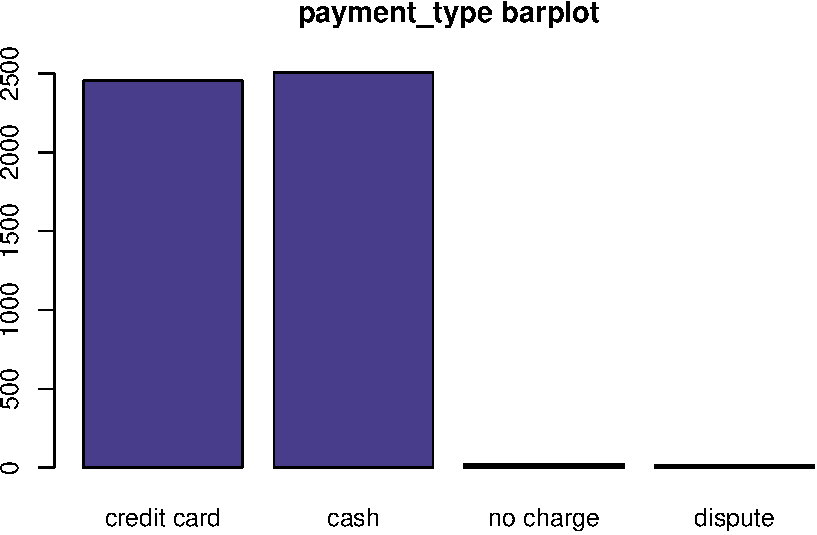
\includegraphics{deliverable1-fixed_files/figure-latex/unnamed-chunk-11-1.pdf}

\hypertarget{ratecodeid}{%
\subsubsection{8. RateCodeID}\label{ratecodeid}}

This variable expresses the different RateCodeIDs that we can have as
numerical values, so we need to categorize them in order to be able to
work with them.

\begin{Shaded}
\begin{Highlighting}[]
\CommentTok{# summary(df$RateCodeID)}
\NormalTok{df}\OperatorTok{$}\NormalTok{RateCodeID<-}\KeywordTok{factor}\NormalTok{(df}\OperatorTok{$}\NormalTok{RateCodeID)}
\KeywordTok{barplot}\NormalTok{(}\KeywordTok{summary}\NormalTok{(df}\OperatorTok{$}\NormalTok{RateCodeID),}\DataTypeTok{main=}\StringTok{"RateCodeID Barplot"}\NormalTok{,}\DataTypeTok{col =} \StringTok{"DarkSlateBlue"}\NormalTok{)}
\end{Highlighting}
\end{Shaded}

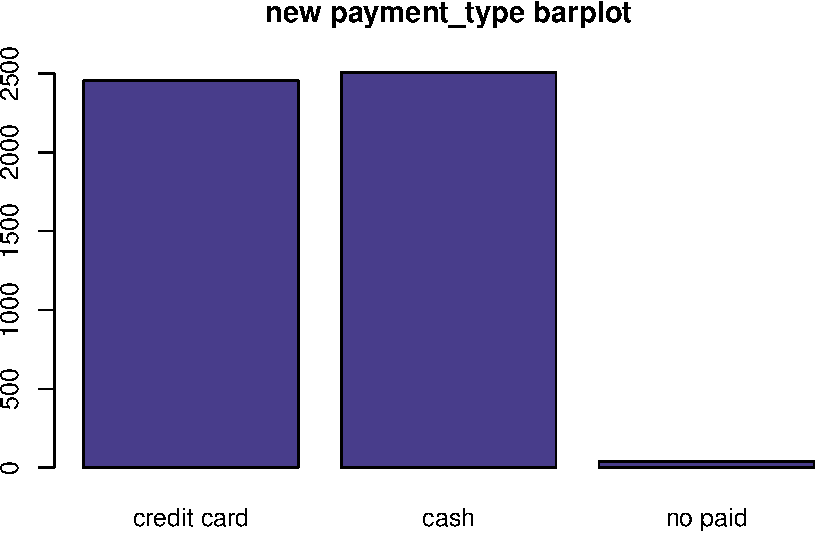
\includegraphics{deliverable1-fixed_files/figure-latex/unnamed-chunk-12-1.pdf}

We see that most samples are in RateCodeID = 1, which is what we are
interested in. Therefore, we factorize and create only two groups, the
one with RateCodeID = 1 and the rest.

\begin{Shaded}
\begin{Highlighting}[]
\NormalTok{df}\OperatorTok{$}\NormalTok{RateCodeID[df}\OperatorTok{$}\NormalTok{RateCodeID }\OperatorTok{!=}\StringTok{ }\DecValTok{1}\NormalTok{] =}\StringTok{ }\DecValTok{2}
\NormalTok{df}\OperatorTok{$}\NormalTok{RateCodeID <-}\StringTok{ }\KeywordTok{factor}\NormalTok{(df}\OperatorTok{$}\NormalTok{RateCodeID, }\DataTypeTok{labels =}\KeywordTok{c}\NormalTok{(}\StringTok{"Rate-1"}\NormalTok{,}\StringTok{"Rate-Other"}\NormalTok{))}
\KeywordTok{barplot}\NormalTok{(}\KeywordTok{summary}\NormalTok{(df}\OperatorTok{$}\NormalTok{RateCodeID),}\DataTypeTok{main=}\StringTok{"RateCodeID Barplot"}\NormalTok{,}\DataTypeTok{col =} \StringTok{"DarkSlateBlue"}\NormalTok{)}
\end{Highlighting}
\end{Shaded}

\includegraphics{deliverable1-fixed_files/figure-latex/unnamed-chunk-13-1.pdf}
Now is more balanced.

\hypertarget{store_and_fwd_flag}{%
\subsubsection{9. Store\_and\_fwd\_flag}\label{store_and_fwd_flag}}

This is a categorical variable with the values Y and N, so we need to
factor it.

\begin{Shaded}
\begin{Highlighting}[]
\CommentTok{# summary(df$Store_and_fwd_flag)}
\NormalTok{df}\OperatorTok{$}\NormalTok{Store_and_fwd_flag<-}\KeywordTok{factor}\NormalTok{(df}\OperatorTok{$}\NormalTok{Store_and_fwd_flag)}
\KeywordTok{barplot}\NormalTok{(}\KeywordTok{summary}\NormalTok{(df}\OperatorTok{$}\NormalTok{Store_and_fwd_flag),}\DataTypeTok{main=}\StringTok{"Store_and_fwd_flag Barplot"}\NormalTok{,}\DataTypeTok{col =} \StringTok{"DarkSlateBlue"}\NormalTok{)}
\end{Highlighting}
\end{Shaded}

\includegraphics{deliverable1-fixed_files/figure-latex/unnamed-chunk-14-1.pdf}

\hypertarget{payment_type}{%
\subsubsection{12. Payment\_type}\label{payment_type}}

This variable is categorical but it is expressed as numerical, so we
need to factor it in order to be able to work with it.

\begin{Shaded}
\begin{Highlighting}[]
\NormalTok{df}\OperatorTok{$}\NormalTok{Payment_type<-}\KeywordTok{factor}\NormalTok{(df}\OperatorTok{$}\NormalTok{Payment_type,}\DataTypeTok{labels=}\KeywordTok{c}\NormalTok{(}\StringTok{"Credit card"}\NormalTok{,}\StringTok{"Cash"}\NormalTok{,}\StringTok{"No charge"}\NormalTok{,}\StringTok{"Dispute"}\NormalTok{))}
\CommentTok{# summary(df$Payment_type)}
\KeywordTok{barplot}\NormalTok{(}\KeywordTok{summary}\NormalTok{(df}\OperatorTok{$}\NormalTok{Payment_type),}\DataTypeTok{main=}\StringTok{"Payment_type Barplot"}\NormalTok{,}\DataTypeTok{col =} \StringTok{"DarkSlateBlue"}\NormalTok{)}
\end{Highlighting}
\end{Shaded}

\includegraphics{deliverable1-fixed_files/figure-latex/unnamed-chunk-15-1.pdf}

As we can see, there are few values with ``No charge'' or ``Dispute''
category, so we decided to categorize it into a new category (``No
paid'').

\begin{Shaded}
\begin{Highlighting}[]
\KeywordTok{levels}\NormalTok{(df}\OperatorTok{$}\NormalTok{Payment_type) <-}\StringTok{ }\KeywordTok{c}\NormalTok{(}\StringTok{"Credit card"}\NormalTok{,}\StringTok{"Cash"}\NormalTok{,}\StringTok{"No paid"}\NormalTok{,}\StringTok{"No paid"}\NormalTok{)}
\CommentTok{# summary(df$Payment_type)}
\KeywordTok{barplot}\NormalTok{(}\KeywordTok{summary}\NormalTok{(df}\OperatorTok{$}\NormalTok{Payment_type),}\DataTypeTok{main=}\StringTok{"Payment_type Barplot"}\NormalTok{,}\DataTypeTok{col =} \StringTok{"DarkSlateBlue"}\NormalTok{)}
\end{Highlighting}
\end{Shaded}

\includegraphics{deliverable1-fixed_files/figure-latex/unnamed-chunk-16-1.pdf}

\hypertarget{trip_type}{%
\subsubsection{21. Trip\_type}\label{trip_type}}

This variable is categorical but it is expressed as numerical, so we
need to factor it in order to be able to work with it.

\begin{Shaded}
\begin{Highlighting}[]
\NormalTok{df}\OperatorTok{$}\NormalTok{Trip_type<-}\KeywordTok{factor}\NormalTok{(df}\OperatorTok{$}\NormalTok{Trip_type,}\DataTypeTok{labels=}\KeywordTok{c}\NormalTok{(}\StringTok{"Street-Hail"}\NormalTok{,}\StringTok{"Dispatch"}\NormalTok{))}
\KeywordTok{barplot}\NormalTok{(}\KeywordTok{summary}\NormalTok{(df}\OperatorTok{$}\NormalTok{Trip_type),}\DataTypeTok{main=}\StringTok{"Trip_type Barplot"}\NormalTok{,}\DataTypeTok{col =} \StringTok{"DarkSlateBlue"}\NormalTok{)}
\end{Highlighting}
\end{Shaded}

\includegraphics{deliverable1-fixed_files/figure-latex/unnamed-chunk-17-1.pdf}

\begin{Shaded}
\begin{Highlighting}[]
\CommentTok{# summary(df$Trip_type)}
\end{Highlighting}
\end{Shaded}

\hypertarget{quantitative-variables}{%
\subsection{Quantitative Variables}\label{quantitative-variables}}

\textbf{Description}: Original numeric variables corresponding to real
quantitative concepts are kept as numeric but additional factors should
also be created as a discretization of each numeric variable.

We only keep the hours (variables 2 and 3) to be able to work with time
slots in the future.

Create new variables derived from the original ones, as effective speed,
travel time, hour of request, period of request, effective trip distance
(in km)

\hypertarget{new-variables-trip-length-in-km-travel-time-un-min-and-effective-speed}{%
\subsubsection{New variables: Trip Length in km, Travel time un min and
Effective
speed}\label{new-variables-trip-length-in-km-travel-time-un-min-and-effective-speed}}

\hypertarget{trip-length-in-km}{%
\paragraph{Trip length in km}\label{trip-length-in-km}}

\begin{Shaded}
\begin{Highlighting}[]
\NormalTok{df}\OperatorTok{$}\NormalTok{tlenkm<-df}\OperatorTok{$}\NormalTok{Trip_distance}\OperatorTok{*}\FloatTok{1.609344} \CommentTok{# Miles to km}
\end{Highlighting}
\end{Shaded}

\hypertarget{travel-time-in-min}{%
\paragraph{Travel time in min}\label{travel-time-in-min}}

\begin{Shaded}
\begin{Highlighting}[]
\NormalTok{df}\OperatorTok{$}\NormalTok{traveltime<-(}\KeywordTok{as.numeric}\NormalTok{(}\KeywordTok{as.POSIXct}\NormalTok{(df}\OperatorTok{$}\NormalTok{Lpep_dropoff_datetime)) }\OperatorTok{-}\StringTok{ }\KeywordTok{as.numeric}\NormalTok{(}\KeywordTok{as.POSIXct}\NormalTok{(df}\OperatorTok{$}\NormalTok{lpep_pickup_datetime)))}\OperatorTok{/}\DecValTok{60}
\end{Highlighting}
\end{Shaded}

\hypertarget{effective-speed-in-kmh}{%
\paragraph{Effective speed in km/h}\label{effective-speed-in-kmh}}

\begin{Shaded}
\begin{Highlighting}[]
\NormalTok{df}\OperatorTok{$}\NormalTok{espeed<-(df}\OperatorTok{$}\NormalTok{tlenkm}\OperatorTok{/}\NormalTok{(df}\OperatorTok{$}\NormalTok{traveltime))}\OperatorTok{*}\DecValTok{60}
\end{Highlighting}
\end{Shaded}

\hypertarget{missing-data}{%
\paragraph{Missing data}\label{missing-data}}

\begin{Shaded}
\begin{Highlighting}[]
\NormalTok{sel<-}\KeywordTok{which}\NormalTok{(}\KeywordTok{is.na}\NormalTok{(df}\OperatorTok{$}\NormalTok{espeed}\OperatorTok{<=}\DecValTok{0}\NormalTok{)) }\CommentTok{#;length(sel)}
\NormalTok{imis[sel]<-imis[sel]}\OperatorTok{+}\DecValTok{1}
\NormalTok{jmis[}\DecValTok{26}\NormalTok{]<-}\KeywordTok{length}\NormalTok{(sel)}
\end{Highlighting}
\end{Shaded}

\hypertarget{error-detection}{%
\paragraph{Error detection}\label{error-detection}}

We detect as error those speeds smaller than 0 and bigger than 200

\begin{Shaded}
\begin{Highlighting}[]
\KeywordTok{summary}\NormalTok{(df}\OperatorTok{$}\NormalTok{espeed)}
\end{Highlighting}
\end{Shaded}

\begin{verbatim}
##    Min. 1st Qu.  Median    Mean 3rd Qu.    Max.    NA's 
##    0.00   14.60   18.58   23.07   23.70 3881.74       2
\end{verbatim}

\begin{Shaded}
\begin{Highlighting}[]
\NormalTok{sel<-}\KeywordTok{which}\NormalTok{((df}\OperatorTok{$}\NormalTok{espeed}\OperatorTok{<=}\DecValTok{0}\NormalTok{)}\OperatorTok{|}\NormalTok{(df}\OperatorTok{$}\NormalTok{espeed }\OperatorTok{>}\StringTok{ }\DecValTok{200}\NormalTok{))}
\NormalTok{ierrs[sel]<-ierrs[sel]}\OperatorTok{+}\DecValTok{1}
\NormalTok{jerrs[}\DecValTok{26}\NormalTok{]<-}\KeywordTok{length}\NormalTok{(sel)}
\CommentTok{# sel}
\end{Highlighting}
\end{Shaded}

Sel contains the rownames of the individuals with ``0'' as value for
longitude

\begin{Shaded}
\begin{Highlighting}[]
\NormalTok{df[sel,}\StringTok{"espeed"}\NormalTok{]<-}\OtherTok{NA} 
\end{Highlighting}
\end{Shaded}

\hypertarget{check-outliers}{%
\paragraph{Check outliers}\label{check-outliers}}

\begin{Shaded}
\begin{Highlighting}[]
\CommentTok{# summary(df$espeed)}
\KeywordTok{calcQ}\NormalTok{(df}\OperatorTok{$}\NormalTok{espeed)}
\end{Highlighting}
\end{Shaded}

\begin{verbatim}
## $souti
##   1st Qu. 
## -12.00637 
## 
## $mouti
##  1st Qu. 
## 1.394097 
## 
## $min
##       Min. 
## 0.03530885 
## 
## $q1
##  1st Qu. 
## 14.79457 
## 
## $q2
##   Median 
## 18.65269 
## 
## $q3
##  3rd Qu. 
## 23.72821 
## 
## $max
##    Max. 
## 144.841 
## 
## $mouts
##  3rd Qu. 
## 37.12868 
## 
## $souts
##  3rd Qu. 
## 50.52915
\end{verbatim}

\hypertarget{outlier-detection}{%
\paragraph{Outlier detection}\label{outlier-detection}}

\begin{Shaded}
\begin{Highlighting}[]
\KeywordTok{Boxplot}\NormalTok{(df}\OperatorTok{$}\NormalTok{espeed)}
\end{Highlighting}
\end{Shaded}

\begin{verbatim}
##  [1] 4780 3001 3066 1936  120 3578 1767 4824 2685 3009 2647 2804 2546 3865 1702
## [16] 4995 1354 3849  132 2075
\end{verbatim}

\begin{Shaded}
\begin{Highlighting}[]
\NormalTok{var_out<-}\KeywordTok{calcQ}\NormalTok{(df}\OperatorTok{$}\NormalTok{espeed)}
\KeywordTok{abline}\NormalTok{(}\DataTypeTok{h=}\NormalTok{var_out}\OperatorTok{$}\NormalTok{souts,}\DataTypeTok{col=}\StringTok{"red"}\NormalTok{)}
\KeywordTok{abline}\NormalTok{(}\DataTypeTok{h=}\NormalTok{var_out}\OperatorTok{$}\NormalTok{souti,}\DataTypeTok{col=}\StringTok{"red"}\NormalTok{)}
\end{Highlighting}
\end{Shaded}

\includegraphics{deliverable1-fixed_files/figure-latex/unnamed-chunk-25-1.pdf}

\begin{Shaded}
\begin{Highlighting}[]
\NormalTok{llout<-}\KeywordTok{which}\NormalTok{((df}\OperatorTok{$}\NormalTok{espeed}\OperatorTok{<=}\DecValTok{3}\NormalTok{)}\OperatorTok{|}\NormalTok{(df}\OperatorTok{$}\NormalTok{espeed}\OperatorTok{>}\DecValTok{80}\NormalTok{))}
\NormalTok{iouts[llout]<-iouts[llout]}\OperatorTok{+}\DecValTok{1}
\NormalTok{jouts[}\DecValTok{26}\NormalTok{]<-}\KeywordTok{length}\NormalTok{(llout)}
\NormalTok{df[llout,}\StringTok{"espeed"}\NormalTok{]<-}\OtherTok{NA} 
\end{Highlighting}
\end{Shaded}

\hypertarget{lpep_pickup_datetime}{%
\subsubsection{2. lpep\_pickup\_datetime}\label{lpep_pickup_datetime}}

We just keep the hours

\begin{Shaded}
\begin{Highlighting}[]
\NormalTok{df}\OperatorTok{$}\NormalTok{pickup<-}\KeywordTok{substr}\NormalTok{(}\KeywordTok{strptime}\NormalTok{(df}\OperatorTok{$}\NormalTok{lpep_pickup_datetime, }\StringTok{"%Y-%m-%d %H:%M:%S"}\NormalTok{), }\DecValTok{12}\NormalTok{, }\DecValTok{13}\NormalTok{) }\CommentTok{# table(df$pickup)}
\end{Highlighting}
\end{Shaded}

\hypertarget{lpep_dropoff_datetime}{%
\subsubsection{3. lpep\_dropoff\_datetime}\label{lpep_dropoff_datetime}}

We just keep the hours

\begin{Shaded}
\begin{Highlighting}[]
\NormalTok{df}\OperatorTok{$}\NormalTok{dropoff<-}\KeywordTok{substr}\NormalTok{(}\KeywordTok{strptime}\NormalTok{(df}\OperatorTok{$}\NormalTok{Lpep_dropoff_datetime, }\StringTok{"%Y-%m-%d %H:%M:%S"}\NormalTok{), }\DecValTok{12}\NormalTok{, }\DecValTok{13}\NormalTok{) }\CommentTok{# table(df$pickup)}
\end{Highlighting}
\end{Shaded}

\hypertarget{passenger_count}{%
\subsubsection{4. Passenger\_count}\label{passenger_count}}

\begin{Shaded}
\begin{Highlighting}[]
\KeywordTok{summary}\NormalTok{(df}\OperatorTok{$}\NormalTok{Passenger_count)}
\end{Highlighting}
\end{Shaded}

\begin{verbatim}
##    Min. 1st Qu.  Median    Mean 3rd Qu.    Max. 
##   0.000   1.000   1.000   1.375   1.000   6.000
\end{verbatim}

We set the 0 as an error because it is not possible to have a trip
without passengers

\begin{Shaded}
\begin{Highlighting}[]
\NormalTok{sel<-}\KeywordTok{which}\NormalTok{(df}\OperatorTok{$}\NormalTok{Passenger_count }\OperatorTok{==}\StringTok{ }\DecValTok{0}\NormalTok{)}
\NormalTok{ierrs[sel]<-ierrs[sel]}\OperatorTok{+}\DecValTok{1}
\CommentTok{# names(df)}
\NormalTok{jerrs[}\DecValTok{10}\NormalTok{]<-}\KeywordTok{length}\NormalTok{(sel)}
\CommentTok{# sel}
\end{Highlighting}
\end{Shaded}

Sel contains the rownames of the individuals with ``0'' as value for
passengers

\begin{Shaded}
\begin{Highlighting}[]
\NormalTok{df[sel,}\StringTok{"Passenger_count"}\NormalTok{]<-}\OtherTok{NA}
\end{Highlighting}
\end{Shaded}

\hypertarget{trip_distance}{%
\subsubsection{5. Trip\_distance}\label{trip_distance}}

\begin{Shaded}
\begin{Highlighting}[]
\KeywordTok{summary}\NormalTok{(df}\OperatorTok{$}\NormalTok{Trip_distance)}
\end{Highlighting}
\end{Shaded}

\begin{verbatim}
##    Min. 1st Qu.  Median    Mean 3rd Qu.    Max. 
##   0.000   1.020   1.800   2.765   3.420  52.790
\end{verbatim}

We see on the summary that there are not NA values, so we proceed to the
outlier and error detection.

\hypertarget{outlier-detection-1}{%
\paragraph{Outlier detection}\label{outlier-detection-1}}

In order to evalute or data, we decide to set the maximum trip distance
to 30, so we proceed to delete the outliers.

\begin{Shaded}
\begin{Highlighting}[]
\KeywordTok{Boxplot}\NormalTok{(df}\OperatorTok{$}\NormalTok{Trip_distance)}
\end{Highlighting}
\end{Shaded}

\begin{verbatim}
##  [1] 2680 4072 1702 2075  723 3107 2691 1105 4301 3154
\end{verbatim}

\begin{Shaded}
\begin{Highlighting}[]
\NormalTok{var_out<-}\KeywordTok{calcQ}\NormalTok{(df}\OperatorTok{$}\NormalTok{Trip_distance)}
\KeywordTok{abline}\NormalTok{(}\DataTypeTok{h=}\NormalTok{var_out}\OperatorTok{$}\NormalTok{souts,}\DataTypeTok{col=}\StringTok{"red"}\NormalTok{)}
\KeywordTok{abline}\NormalTok{(}\DataTypeTok{h=}\NormalTok{var_out}\OperatorTok{$}\NormalTok{souti,}\DataTypeTok{col=}\StringTok{"red"}\NormalTok{)}
\KeywordTok{abline}\NormalTok{(}\DataTypeTok{h=}\DecValTok{30}\NormalTok{,}\DataTypeTok{col=}\StringTok{"blue"}\NormalTok{,}\DataTypeTok{lwd=}\DecValTok{2}\NormalTok{)}
\end{Highlighting}
\end{Shaded}

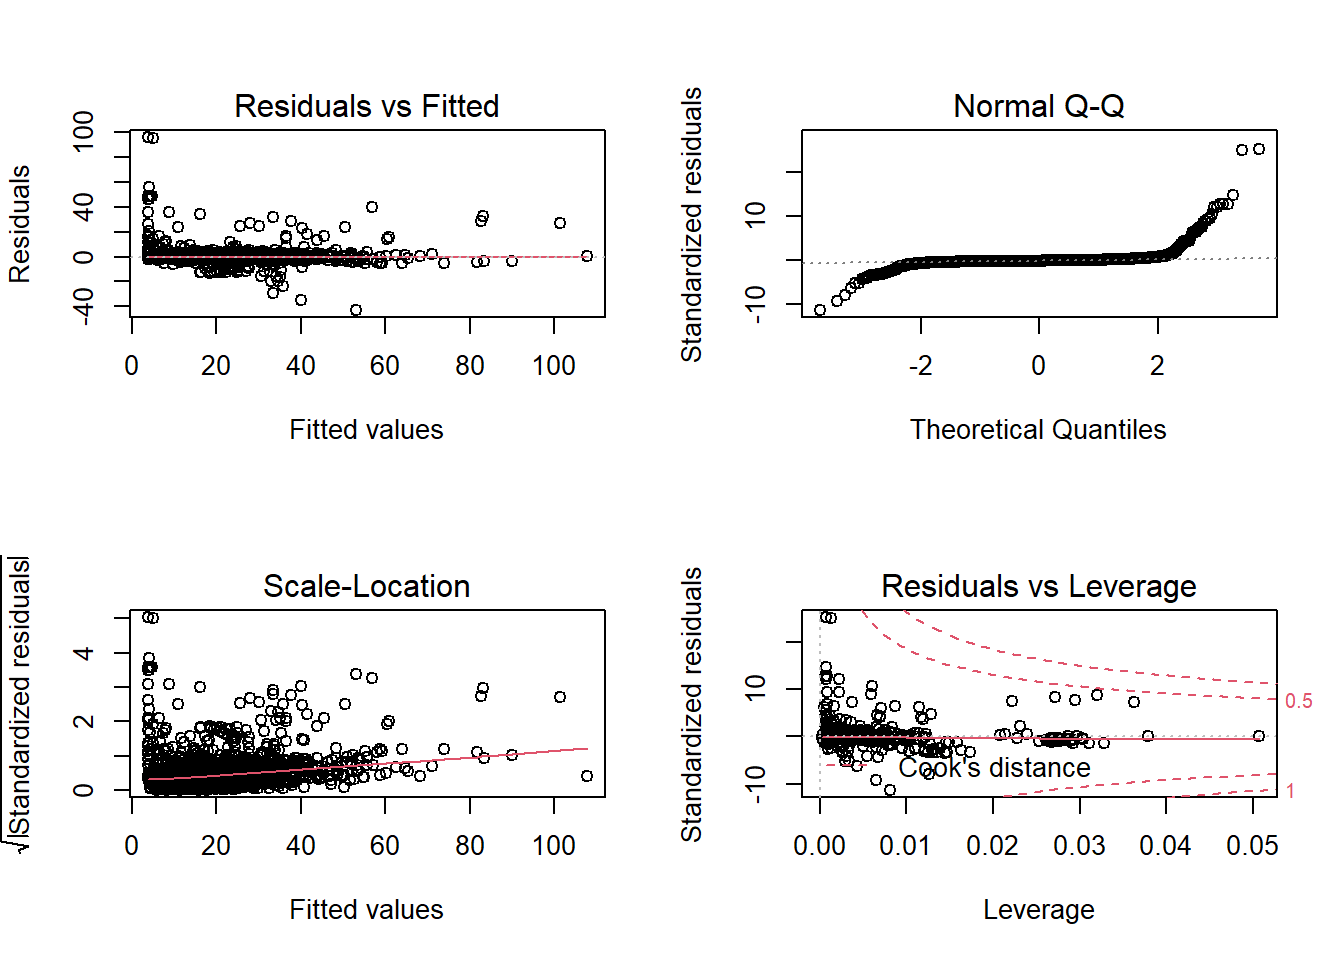
\includegraphics{deliverable1-fixed_files/figure-latex/unnamed-chunk-32-1.pdf}

\begin{Shaded}
\begin{Highlighting}[]
\NormalTok{llout<-}\KeywordTok{which}\NormalTok{(df}\OperatorTok{$}\NormalTok{Trip_distance}\OperatorTok{>}\DecValTok{30}\NormalTok{)}
\NormalTok{iouts[llout]<-iouts[llout]}\OperatorTok{+}\DecValTok{1}
\CommentTok{# names(df)}
\NormalTok{jouts[}\DecValTok{11}\NormalTok{]<-}\KeywordTok{length}\NormalTok{(llout)}
\end{Highlighting}
\end{Shaded}

\hypertarget{error-detection-1}{%
\paragraph{Error detection}\label{error-detection-1}}

We decide that an incorrect trip distance is the one with 0 miles or
less. In order to be aware of this error we store it at ierrs, and
jerrs. ierrs stores the number of errors in a row, and jerrs stores the
total amount of errors in a variable.

\begin{Shaded}
\begin{Highlighting}[]
\NormalTok{sel<-}\KeywordTok{which}\NormalTok{(df}\OperatorTok{$}\NormalTok{Trip_distance }\OperatorTok{<=}\StringTok{ }\DecValTok{0}\NormalTok{)}
\NormalTok{ierrs[sel]<-ierrs[sel]}\OperatorTok{+}\DecValTok{1}
\CommentTok{# names(df)}
\NormalTok{jerrs[}\DecValTok{11}\NormalTok{]<-}\KeywordTok{length}\NormalTok{(sel)}
\CommentTok{# sel }
\end{Highlighting}
\end{Shaded}

\hypertarget{errors-and-outliers}{%
\paragraph{Errors and outliers}\label{errors-and-outliers}}

Now, we set NA values in order to remove errors and outliersfrom the
dataset

\begin{Shaded}
\begin{Highlighting}[]
\NormalTok{setNA<-}\KeywordTok{which}\NormalTok{((df}\OperatorTok{$}\NormalTok{Trip_distance}\OperatorTok{<=}\DecValTok{0}\NormalTok{) }\OperatorTok{|}\StringTok{ }\NormalTok{(df}\OperatorTok{$}\NormalTok{Trip_distance }\OperatorTok{>}\StringTok{ }\DecValTok{30}\NormalTok{))}
\NormalTok{df[setNA,}\StringTok{"Trip_distance"}\NormalTok{]<-}\OtherTok{NA}
\end{Highlighting}
\end{Shaded}

\hypertarget{caterogial-variable-for-trip_distance}{%
\paragraph{Caterogial variable for
Trip\_distance}\label{caterogial-variable-for-trip_distance}}

We are going to set a categorical variable for the Trip\_distancerange.
We decided to create 3 levels: ``Short\_dist'', ``Medium\_dist''
and``Long\_dist''. - Short\_dist \textless= 2.5 - Medium\_dist 2.5
\textless{} Trip\_distance \textless= 5 - Long\_dist \textgreater{} 5

\begin{Shaded}
\begin{Highlighting}[]
\NormalTok{df}\OperatorTok{$}\NormalTok{Trip_distance_range[df}\OperatorTok{$}\NormalTok{Trip_distance }\OperatorTok{<=}\StringTok{ }\FloatTok{2.5}\NormalTok{] =}\StringTok{ "Short_dist"}
\NormalTok{df}\OperatorTok{$}\NormalTok{Trip_distance_range[(df}\OperatorTok{$}\NormalTok{Trip_distance }\OperatorTok{>}\StringTok{ }\FloatTok{2.5}\NormalTok{) }\OperatorTok{&}\StringTok{ }\NormalTok{(df}\OperatorTok{$}\NormalTok{Trip_distance }\OperatorTok{<=}\StringTok{ }\DecValTok{5}\NormalTok{)] =}\StringTok{ "Medium_dist"}
\NormalTok{df}\OperatorTok{$}\NormalTok{Trip_distance_range[df}\OperatorTok{$}\NormalTok{Trip_distance }\OperatorTok{>}\StringTok{ }\DecValTok{5}\NormalTok{] =}\StringTok{ "Long_dist"}
\CommentTok{# summary(df$Trip_distance_range)}
\end{Highlighting}
\end{Shaded}

We see, though, that it is not a factor yet, so we factor it.

\begin{Shaded}
\begin{Highlighting}[]
\NormalTok{df}\OperatorTok{$}\NormalTok{Trip_distance_range <-}\StringTok{ }\KeywordTok{factor}\NormalTok{(df}\OperatorTok{$}\NormalTok{Trip_distance_range)}
\end{Highlighting}
\end{Shaded}

We see a barplot for the factor we created.

\begin{Shaded}
\begin{Highlighting}[]
\KeywordTok{barplot}\NormalTok{(}\KeywordTok{table}\NormalTok{(df}\OperatorTok{$}\NormalTok{Trip_distance_range),}\DataTypeTok{main=}\StringTok{"Trip_distance_range Barplot"}\NormalTok{,}\DataTypeTok{col =} \StringTok{"DarkSlateBlue"}\NormalTok{)}
\end{Highlighting}
\end{Shaded}

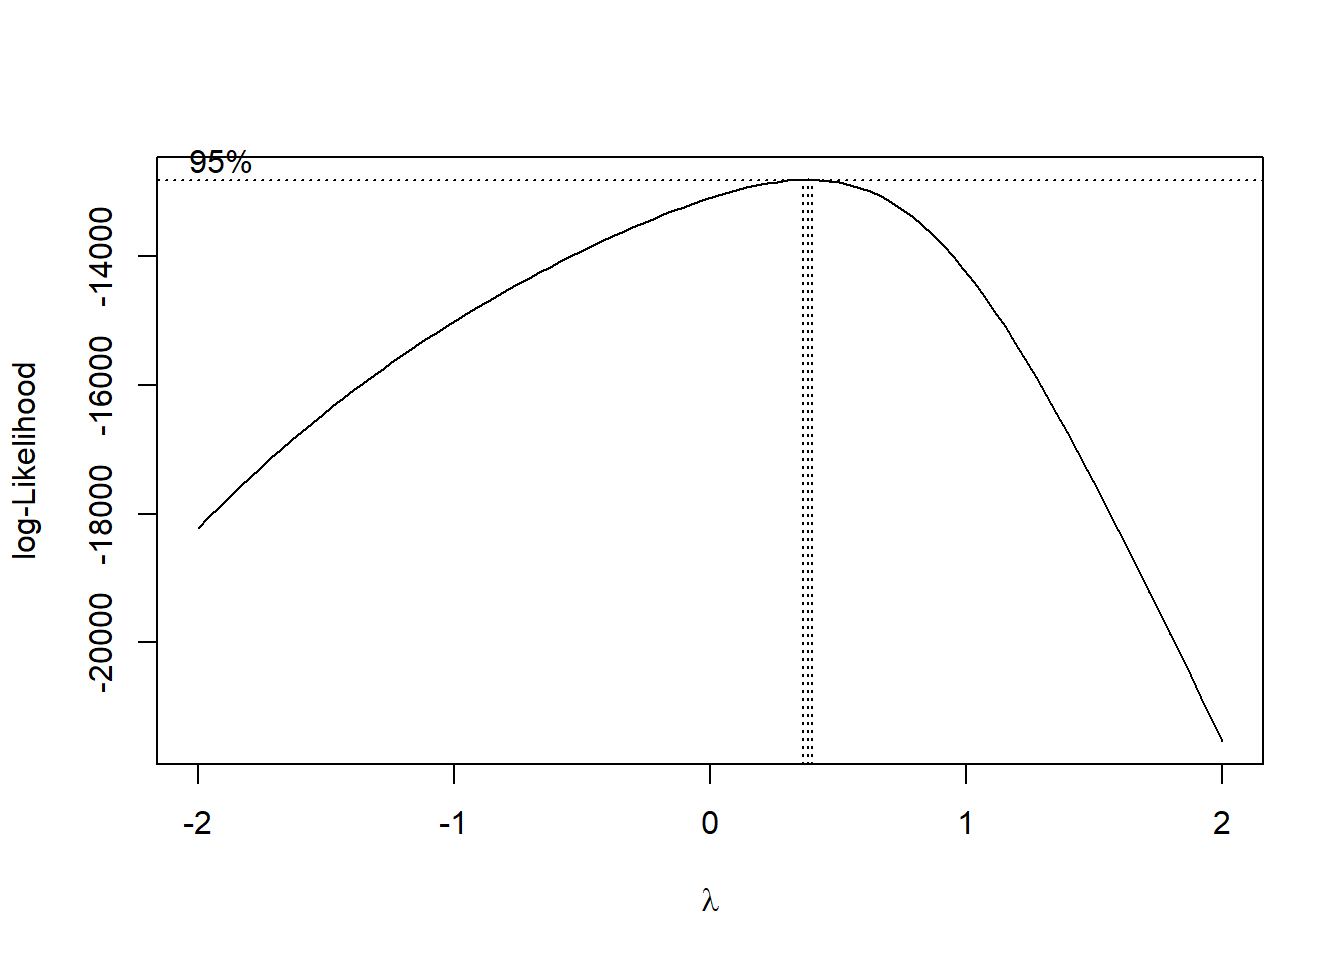
\includegraphics{deliverable1-fixed_files/figure-latex/unnamed-chunk-37-1.pdf}

\hypertarget{pickup_longitude}{%
\subsubsection{6. Pickup\_longitude}\label{pickup_longitude}}

We know that New York's longitude is -73.9385, so values that differ a
lot from this value is an error or an outlier.

\begin{Shaded}
\begin{Highlighting}[]
\KeywordTok{summary}\NormalTok{(df}\OperatorTok{$}\NormalTok{Pickup_longitude)}
\end{Highlighting}
\end{Shaded}

\begin{verbatim}
##    Min. 1st Qu.  Median    Mean 3rd Qu.    Max. 
##  -75.39  -73.96  -73.95  -73.89  -73.92    0.00
\end{verbatim}

0.00 looks to be an error Seeing the individuals with this ``0'' value:
df{[}which(df{[},``Pickup\_longitude''{]}==0),{]} it is a quantitive
variable. Non-possible values will be recoded as errors, so will be
transformed to NA.

\begin{Shaded}
\begin{Highlighting}[]
\NormalTok{sel<-}\KeywordTok{which}\NormalTok{(df}\OperatorTok{$}\NormalTok{Pickup_longitude }\OperatorTok{==}\StringTok{ }\DecValTok{0}\NormalTok{)}
\NormalTok{ierrs[sel]<-ierrs[sel]}\OperatorTok{+}\DecValTok{1}
\CommentTok{# names(df)}
\NormalTok{jerrs[}\DecValTok{6}\NormalTok{]<-}\KeywordTok{length}\NormalTok{(sel)}
\CommentTok{# sel  }
\end{Highlighting}
\end{Shaded}

Sel contains the rownames of the individuals with ``0'' as value for
longitude.

\begin{Shaded}
\begin{Highlighting}[]
\NormalTok{df[sel,}\StringTok{"Pickup_longitude"}\NormalTok{]<-}\OtherTok{NA}   
\end{Highlighting}
\end{Shaded}

Non-possible values are replaced by NA, missing value symbol in R.

\hypertarget{which-trips-are-not-running-in-new-york}{%
\paragraph{Which trips are not running in
New-York?}\label{which-trips-are-not-running-in-new-york}}

Consider if, at least, one of the pick-up and drop-off points belong to
New-York area. if not, this trip is an ``out-of-scope'' individual and
has to be eliminated of the basis. Nevertheless, you have to justify
thiselimination and count how many individuals were in this situation.
Look at that!! possibly, starting from the outliers\ldots{}``0'' is
missing value, outliers can help to detect trips running outside of New
York\ldots{}

We are deleting trips from outside New York. This means we are not using
longitudes bigger than -73.80 and smaller than -74.02.

\begin{Shaded}
\begin{Highlighting}[]
\NormalTok{llout <-}\KeywordTok{which}\NormalTok{((df}\OperatorTok{$}\NormalTok{Pickup_longitude }\OperatorTok{<}\StringTok{ }\FloatTok{-74.02}\NormalTok{) }\OperatorTok{|}\StringTok{ }\NormalTok{(df}\OperatorTok{$}\NormalTok{Pickup_longitude }\OperatorTok{>}\StringTok{ }\FloatTok{-73.80}\NormalTok{))}
\NormalTok{iouts[llout]<-iouts[llout]}\OperatorTok{+}\DecValTok{1}
\CommentTok{# names(df)}
\NormalTok{jouts[}\DecValTok{6}\NormalTok{]<-}\KeywordTok{length}\NormalTok{(llout)}
\end{Highlighting}
\end{Shaded}

Now that we have the outliers, we are setting them as NA

\begin{Shaded}
\begin{Highlighting}[]
\NormalTok{df[llout,}\StringTok{"Pickup_longitude"}\NormalTok{]<-}\OtherTok{NA}
\end{Highlighting}
\end{Shaded}

\hypertarget{pickup_latitude}{%
\subsubsection{7. Pickup\_latitude}\label{pickup_latitude}}

We know that New York's latitude is 40.6643, so values that differ a lot
from this value is an error or an outlier.

\begin{Shaded}
\begin{Highlighting}[]
\KeywordTok{summary}\NormalTok{(df}\OperatorTok{$}\NormalTok{Pickup_latitude)}
\end{Highlighting}
\end{Shaded}

\begin{verbatim}
##    Min. 1st Qu.  Median    Mean 3rd Qu.    Max. 
##    0.00   40.70   40.75   40.72   40.80   41.04
\end{verbatim}

0.00 looks to be an error. Seeing the individuals with this ``0'' value:
df{[}which(df{[},``Pickup\_latitude''{]}==0),{]} it is a quantitive
variable. non-possible values will be recoded as errors, so will be
transformed to NA.

\begin{Shaded}
\begin{Highlighting}[]
\NormalTok{sel<-}\KeywordTok{which}\NormalTok{(df}\OperatorTok{$}\NormalTok{Pickup_latitude }\OperatorTok{==}\StringTok{ }\DecValTok{0}\NormalTok{)}
\NormalTok{ierrs[sel]<-ierrs[sel]}\OperatorTok{+}\DecValTok{1}
\CommentTok{# names(df)}
\NormalTok{jerrs[}\DecValTok{7}\NormalTok{]<-}\KeywordTok{length}\NormalTok{(sel)}
\CommentTok{# sel  }
\end{Highlighting}
\end{Shaded}

Sel contains the rownames of the individuals with ``0'' as value for
longitude

\begin{Shaded}
\begin{Highlighting}[]
\NormalTok{df[sel,}\StringTok{"Pickup_longitude"}\NormalTok{]<-}\OtherTok{NA}  
\end{Highlighting}
\end{Shaded}

Non-possible values are replaced by NA, missing value symbol in R. We
are deleting trips from outside New York. This means we are not using
latitudes bigger than 40.54 and smallerthan 40.86

\begin{Shaded}
\begin{Highlighting}[]
\NormalTok{llout <-}\KeywordTok{which}\NormalTok{((df}\OperatorTok{$}\NormalTok{Pickup_latitude }\OperatorTok{<}\StringTok{ }\FloatTok{40.54}\NormalTok{) }\OperatorTok{|}\StringTok{ }\NormalTok{(df}\OperatorTok{$}\NormalTok{Pickup_latitude }\OperatorTok{>}\StringTok{ }\FloatTok{40.86}\NormalTok{))}
\NormalTok{iouts[llout]<-iouts[llout]}\OperatorTok{+}\DecValTok{1}
\CommentTok{# names(df)}
\NormalTok{jouts[}\DecValTok{7}\NormalTok{]<-}\KeywordTok{length}\NormalTok{(llout)}
\end{Highlighting}
\end{Shaded}

Now that we have the outliers, we are setting them as NA

\begin{Shaded}
\begin{Highlighting}[]
\NormalTok{df[llout,}\StringTok{"Pickup_latitude"}\NormalTok{]<-}\OtherTok{NA}
\end{Highlighting}
\end{Shaded}

\hypertarget{dropoff_longitude}{%
\subsubsection{10. Dropoff\_longitude}\label{dropoff_longitude}}

We know that New York's longitude is -73.9385, so values that differ a
lot from this value is an error or an outlier.

\begin{Shaded}
\begin{Highlighting}[]
\KeywordTok{summary}\NormalTok{(df}\OperatorTok{$}\NormalTok{Dropoff_longitude)}
\end{Highlighting}
\end{Shaded}

\begin{verbatim}
##    Min. 1st Qu.  Median    Mean 3rd Qu.    Max. 
##  -75.31  -73.97  -73.94  -73.80  -73.91    0.00
\end{verbatim}

0.00 looks to be an error Seeing the individuals with this ``0'' value:
df{[}which(df{[},``Dropoff\_longitude''{]}==0),{]} it is a quantitive
variable.\\
Non-possible values will be recoded as errors, so will be transformed to
NA.

\begin{Shaded}
\begin{Highlighting}[]
\NormalTok{sel<-}\KeywordTok{which}\NormalTok{(df}\OperatorTok{$}\NormalTok{Dropoff_longitude }\OperatorTok{==}\StringTok{ }\DecValTok{0}\NormalTok{)}
\NormalTok{ierrs[sel]<-ierrs[sel]}\OperatorTok{+}\DecValTok{1}
\CommentTok{# names(df)}
\NormalTok{jerrs[}\DecValTok{8}\NormalTok{]<-}\KeywordTok{length}\NormalTok{(sel)}
\CommentTok{# sel  }
\end{Highlighting}
\end{Shaded}

Sel contains the rownames of the individuals with ``0'' as value for
longitude

\begin{Shaded}
\begin{Highlighting}[]
\NormalTok{df[sel,}\StringTok{"Dropoff_longitude"}\NormalTok{]<-}\OtherTok{NA} 
\end{Highlighting}
\end{Shaded}

Non-possible values are replaced by NA, missing value symbol in R. We
are deleting trips from outside New York. This means we are not using
longitudes bigger than -73.80 and smaller than -74.02.

\begin{Shaded}
\begin{Highlighting}[]
\NormalTok{llout <-}\KeywordTok{which}\NormalTok{((df}\OperatorTok{$}\NormalTok{Dropoff_longitude }\OperatorTok{<}\StringTok{ }\FloatTok{-74.02}\NormalTok{) }\OperatorTok{|}\StringTok{ }\NormalTok{(df}\OperatorTok{$}\NormalTok{Dropoff_longitude }\OperatorTok{>}\StringTok{ }\FloatTok{-73.80}\NormalTok{))}
\NormalTok{iouts[llout]<-iouts[llout]}\OperatorTok{+}\DecValTok{1}
\CommentTok{# names(df)}
\NormalTok{jouts[}\DecValTok{8}\NormalTok{]<-}\KeywordTok{length}\NormalTok{(llout)}
\CommentTok{# llout}
\end{Highlighting}
\end{Shaded}

Now that we have the outliers, we are setting them as NA

\begin{Shaded}
\begin{Highlighting}[]
\NormalTok{df[llout,}\StringTok{"Dropoff_longitude"}\NormalTok{]<-}\OtherTok{NA}
\end{Highlighting}
\end{Shaded}

\hypertarget{dropoff_latitude}{%
\subsubsection{11. Dropoff\_latitude}\label{dropoff_latitude}}

We know that New York's latitude is 40.6643, so values that differ a lot
from this value is an error or an outlier.

\begin{Shaded}
\begin{Highlighting}[]
\KeywordTok{summary}\NormalTok{(df}\OperatorTok{$}\NormalTok{Dropoff_latitude)}
\end{Highlighting}
\end{Shaded}

\begin{verbatim}
##    Min. 1st Qu.  Median    Mean 3rd Qu.    Max. 
##    0.00   40.70   40.75   40.67   40.79   41.18
\end{verbatim}

0.00 looks to be an error Seeing the individuals with this ``0'' value:
df{[}which(df{[},``Dropoff\_latitude''{]}==0),{]} it is a quantitive
variable. Non-possible values will be recoded as errors, so will be
transformed to NA.

\begin{Shaded}
\begin{Highlighting}[]
\NormalTok{sel<-}\KeywordTok{which}\NormalTok{(df}\OperatorTok{$}\NormalTok{Dropoff_latitude }\OperatorTok{==}\StringTok{ }\DecValTok{0}\NormalTok{)}
\NormalTok{ierrs[sel]<-ierrs[sel]}\OperatorTok{+}\DecValTok{1}
\CommentTok{# names(df)}
\NormalTok{jerrs[}\DecValTok{8}\NormalTok{]<-}\KeywordTok{length}\NormalTok{(sel)}
\CommentTok{# sel                }
\end{Highlighting}
\end{Shaded}

Sel contains the rownames of the individuals with ``0'' as value for
longitude

\begin{Shaded}
\begin{Highlighting}[]
\NormalTok{df[sel,}\StringTok{"Dropoff_latitude"}\NormalTok{]<-}\OtherTok{NA}   
\end{Highlighting}
\end{Shaded}

Non-possible values are replaced by NA, missing value symbol in R. We
are deleting trips from outside New York. This means we are not using
latitude bigger than 40.54 and smaller than 40.86

\begin{Shaded}
\begin{Highlighting}[]
\NormalTok{llout <-}\KeywordTok{which}\NormalTok{((df}\OperatorTok{$}\NormalTok{Dropoff_latitude }\OperatorTok{<}\StringTok{ }\FloatTok{40.54}\NormalTok{) }\OperatorTok{|}\StringTok{ }\NormalTok{(df}\OperatorTok{$}\NormalTok{Dropoff_latitude }\OperatorTok{>}\StringTok{ }\FloatTok{40.86}\NormalTok{))}
\NormalTok{iouts[llout]<-iouts[llout]}\OperatorTok{+}\DecValTok{1}
\CommentTok{#names(df)}
\NormalTok{jouts[}\DecValTok{9}\NormalTok{]<-}\KeywordTok{length}\NormalTok{(llout)}
\CommentTok{# llout}
\end{Highlighting}
\end{Shaded}

Now that we have the outliers, we are setting them as NA

\begin{Shaded}
\begin{Highlighting}[]
\NormalTok{df[llout,}\StringTok{"Dropoff_latitude"}\NormalTok{]<-}\OtherTok{NA}
\end{Highlighting}
\end{Shaded}

\hypertarget{fare_amount}{%
\subsubsection{13. Fare\_amount}\label{fare_amount}}

We know that the fare should be positive, as it is the price of the
trip, so we'll treat as error those values. The next we'll do is decide
the outliers.

\begin{Shaded}
\begin{Highlighting}[]
\KeywordTok{summary}\NormalTok{(df}\OperatorTok{$}\NormalTok{Fare_amount)}
\end{Highlighting}
\end{Shaded}

\begin{verbatim}
##    Min. 1st Qu.  Median    Mean 3rd Qu.    Max. 
##   -52.0     6.0     9.0    11.9    14.5   200.0
\end{verbatim}

\begin{Shaded}
\begin{Highlighting}[]
\NormalTok{sel<-}\KeywordTok{which}\NormalTok{(df}\OperatorTok{$}\NormalTok{Fare_amount }\OperatorTok{<=}\StringTok{ }\DecValTok{0}\NormalTok{)}
\NormalTok{ierrs[sel]<-ierrs[sel]}\OperatorTok{+}\DecValTok{1}
\CommentTok{# names(df)}
\NormalTok{jerrs[}\DecValTok{12}\NormalTok{]<-}\KeywordTok{length}\NormalTok{(sel)}
\CommentTok{# sel }
\end{Highlighting}
\end{Shaded}

\begin{Shaded}
\begin{Highlighting}[]
\NormalTok{df[sel,}\StringTok{"Fare_amount"}\NormalTok{]<-}\OtherTok{NA}    
\end{Highlighting}
\end{Shaded}

Non-possible values are replaced by NA, missing value symbol in R

\hypertarget{outlier-detection-2}{%
\paragraph{Outlier detection}\label{outlier-detection-2}}

\begin{Shaded}
\begin{Highlighting}[]
\KeywordTok{Boxplot}\NormalTok{(df}\OperatorTok{$}\NormalTok{Fare_amount)}
\end{Highlighting}
\end{Shaded}

\begin{verbatim}
##  [1]  633  634 2680 4072 1702 4284 2075 2560 3755  723
\end{verbatim}

\begin{Shaded}
\begin{Highlighting}[]
\NormalTok{var_out<-}\KeywordTok{calcQ}\NormalTok{(df}\OperatorTok{$}\NormalTok{Fare_amount)}
\KeywordTok{abline}\NormalTok{(}\DataTypeTok{h=}\NormalTok{var_out}\OperatorTok{$}\NormalTok{souts,}\DataTypeTok{col=}\StringTok{"red"}\NormalTok{)}
\KeywordTok{abline}\NormalTok{(}\DataTypeTok{h=}\NormalTok{var_out}\OperatorTok{$}\NormalTok{souti,}\DataTypeTok{col=}\StringTok{"red"}\NormalTok{)}
\KeywordTok{abline}\NormalTok{(}\DataTypeTok{h=}\DecValTok{60}\NormalTok{,}\DataTypeTok{col=}\StringTok{"blue"}\NormalTok{,}\DataTypeTok{lwd=}\DecValTok{2}\NormalTok{)}
\end{Highlighting}
\end{Shaded}

\includegraphics{deliverable1-fixed_files/figure-latex/unnamed-chunk-61-1.pdf}

We decide to set outliers for fare amounts bigger than 60, because the
majority of the values are concentrated between 0 and 60.

\begin{Shaded}
\begin{Highlighting}[]
\NormalTok{llout<-}\KeywordTok{which}\NormalTok{(df}\OperatorTok{$}\NormalTok{Fare_amount}\OperatorTok{>}\DecValTok{60}\NormalTok{)}
\NormalTok{iouts[llout]<-iouts[llout]}\OperatorTok{+}\DecValTok{1}
\NormalTok{jouts[}\DecValTok{12}\NormalTok{]<-}\KeywordTok{length}\NormalTok{(llout)}
\NormalTok{df[llout,}\StringTok{"Fare_amount"}\NormalTok{]<-}\OtherTok{NA} 
\CommentTok{# llout}
\end{Highlighting}
\end{Shaded}

\hypertarget{extra}{%
\subsubsection{14. Extra}\label{extra}}

As this variable is price related, it cannot have negative values, so
this individuals will be treated as errors.

\begin{Shaded}
\begin{Highlighting}[]
\KeywordTok{summary}\NormalTok{(df}\OperatorTok{$}\NormalTok{Extra)}
\end{Highlighting}
\end{Shaded}

\begin{verbatim}
##    Min. 1st Qu.  Median    Mean 3rd Qu.    Max. 
## -1.0000  0.0000  0.5000  0.3517  0.5000  1.0000
\end{verbatim}

We execute table in order to see every different value in the sample

\begin{Shaded}
\begin{Highlighting}[]
\KeywordTok{table}\NormalTok{(df}\OperatorTok{$}\NormalTok{Extra)}
\end{Highlighting}
\end{Shaded}

\begin{verbatim}
## 
##   -1 -0.5    0  0.5    1 
##    2    5 2296 1868  829
\end{verbatim}

As it is a price related variable, negative values should be treated as
errors, and the other values are the ones defined for this variable, so
there are not outliers.

\begin{Shaded}
\begin{Highlighting}[]
\CommentTok{# df[which(df[, "Extra"] < 0),]}
\NormalTok{sel<-}\KeywordTok{which}\NormalTok{(df}\OperatorTok{$}\NormalTok{Extra }\OperatorTok{<}\StringTok{ }\DecValTok{0}\NormalTok{)}
\NormalTok{ierrs[sel]<-ierrs[sel]}\OperatorTok{+}\DecValTok{1}
\CommentTok{# names(df)}
\NormalTok{jerrs[}\DecValTok{13}\NormalTok{]<-}\KeywordTok{length}\NormalTok{(sel)}
\NormalTok{df[sel,}\StringTok{"Extra"}\NormalTok{]<-}\OtherTok{NA} 
\CommentTok{# sel}
\end{Highlighting}
\end{Shaded}

\hypertarget{mta_tax}{%
\subsubsection{15. MTA\_tax}\label{mta_tax}}

This variable corresponds to a tax that must be charged in every trip
and its cost is \$0.50, so values different from this are errors, and we
don't have to take into account outliers because after the errors
detection all values should be the MTA\_tax.

\begin{Shaded}
\begin{Highlighting}[]
\KeywordTok{summary}\NormalTok{(df}\OperatorTok{$}\NormalTok{MTA_tax)}
\end{Highlighting}
\end{Shaded}

\begin{verbatim}
##    Min. 1st Qu.  Median    Mean 3rd Qu.    Max. 
## -0.5000  0.5000  0.5000  0.4857  0.5000  0.5000
\end{verbatim}

\begin{Shaded}
\begin{Highlighting}[]
\CommentTok{# df[which(df[, "MTA_tax"] != 0.50),]}
\end{Highlighting}
\end{Shaded}

\textbf{Important note:} We assume that when this tax is smaller than 0,
it is an error. If tax is 0, we say that payment in these cases is
equivalent to ``no paid''.

\begin{Shaded}
\begin{Highlighting}[]
\NormalTok{sel<-}\KeywordTok{which}\NormalTok{(df}\OperatorTok{$}\NormalTok{MTA_tax }\OperatorTok{<}\StringTok{ }\DecValTok{0}\NormalTok{)}
\NormalTok{ierrs[sel]<-ierrs[sel]}\OperatorTok{+}\DecValTok{1}
\CommentTok{# names(df)}
\NormalTok{jerrs[}\DecValTok{14}\NormalTok{]<-}\KeywordTok{length}\NormalTok{(sel)}
\NormalTok{df[sel,}\StringTok{"MTA_tax"}\NormalTok{]<-}\OtherTok{NA} 
\CommentTok{# sel}
\end{Highlighting}
\end{Shaded}

\hypertarget{improvement_surcharge}{%
\subsubsection{16. Improvement\_surcharge}\label{improvement_surcharge}}

This variable corresponds to a charge that must be charged in every trip
and its cost is \$0.30, so values smaller than 0 are errors, and we
don't have to take into account outliers because after the errors
detection all values should be the Improvement surcharge.

\begin{Shaded}
\begin{Highlighting}[]
\KeywordTok{summary}\NormalTok{(df}\OperatorTok{$}\NormalTok{improvement_surcharge)}
\end{Highlighting}
\end{Shaded}

\begin{verbatim}
##    Min. 1st Qu.  Median    Mean 3rd Qu.    Max. 
## -0.3000  0.3000  0.3000  0.2914  0.3000  0.3000
\end{verbatim}

\begin{Shaded}
\begin{Highlighting}[]
\KeywordTok{table}\NormalTok{(df}\OperatorTok{$}\NormalTok{improvement_surcharge)}
\end{Highlighting}
\end{Shaded}

\begin{verbatim}
## 
## -0.3    0  0.3 
##   11  121 4868
\end{verbatim}

We know that this surcharge was leived in 2015, so we need to check if
the 0 values correspond to trips before this year. That is what we are
going to do.

\begin{Shaded}
\begin{Highlighting}[]
\NormalTok{df}\OperatorTok{$}\NormalTok{yearGt2015[(df}\OperatorTok{$}\NormalTok{lpep_pickup_datetime }\OperatorTok{>=}\StringTok{ "2015-01-01 00:00:00"}\NormalTok{) }\OperatorTok{&}\StringTok{ }\NormalTok{(df}\OperatorTok{$}\NormalTok{improvement_surcharge }\OperatorTok{==}\StringTok{ }\FloatTok{0.3}\NormalTok{)] =}\StringTok{ }\DecValTok{1}
\NormalTok{df}\OperatorTok{$}\NormalTok{yearGt2015[(df}\OperatorTok{$}\NormalTok{lpep_pickup_datetime }\OperatorTok{<}\StringTok{ "2015-01-01 00:00:00"}\NormalTok{) }\OperatorTok{|}\StringTok{ }\NormalTok{(df}\OperatorTok{$}\NormalTok{improvement_surcharge }\OperatorTok{!=}\StringTok{ }\FloatTok{0.3}\NormalTok{)] =}\StringTok{ }\DecValTok{0}

\KeywordTok{table}\NormalTok{(df}\OperatorTok{$}\NormalTok{yearGt2015)}
\end{Highlighting}
\end{Shaded}

\begin{verbatim}
## 
##    0    1 
##  132 4868
\end{verbatim}

We see that the 0 individuals are errors.

\begin{Shaded}
\begin{Highlighting}[]
\NormalTok{sel<-}\KeywordTok{which}\NormalTok{(df}\OperatorTok{$}\NormalTok{improvement_surcharge }\OperatorTok{<}\StringTok{ }\DecValTok{0}\NormalTok{)}
\NormalTok{ierrs[sel]<-ierrs[sel]}\OperatorTok{+}\DecValTok{1}
\CommentTok{# names(df)}
\NormalTok{jerrs[}\DecValTok{18}\NormalTok{]<-}\KeywordTok{length}\NormalTok{(sel)}
\NormalTok{df[sel,}\StringTok{"improvement_surcharge"}\NormalTok{]<-}\OtherTok{NA} 
\CommentTok{# sel}
\end{Highlighting}
\end{Shaded}

\hypertarget{ehail_fee}{%
\subsubsection{17. Ehail\_fee}\label{ehail_fee}}

We don't take this into account because every value of our sample is NA.

\begin{Shaded}
\begin{Highlighting}[]
\KeywordTok{summary}\NormalTok{(df}\OperatorTok{$}\NormalTok{Ehail_fee)}
\end{Highlighting}
\end{Shaded}

\begin{verbatim}
##    Mode    NA's 
## logical    5000
\end{verbatim}

\hypertarget{tip_amount}{%
\subsubsection{18. Tip\_amount}\label{tip_amount}}

As this is a price related variable, negative values should be
considered as errors, and big tips should be considered as outliers.
Also tip amounts bigger than 0 for individuals with payment\_type =
``Cash'' should be considered as errors as well.

\begin{Shaded}
\begin{Highlighting}[]
\KeywordTok{summary}\NormalTok{(df}\OperatorTok{$}\NormalTok{Tip_amount)}
\end{Highlighting}
\end{Shaded}

\begin{verbatim}
##    Min. 1st Qu.  Median    Mean 3rd Qu.    Max. 
##   0.000   0.000   0.000   1.217   2.000  96.000
\end{verbatim}

We proceed to check if the 0 values are related with payment\_type =
``Credit card'' and the passenger did not tip.

\begin{Shaded}
\begin{Highlighting}[]
\NormalTok{df}\OperatorTok{$}\NormalTok{CashTips[(df}\OperatorTok{$}\NormalTok{Tip_amount }\OperatorTok{>}\StringTok{ }\DecValTok{0}\NormalTok{) }\OperatorTok{&}\StringTok{ }\NormalTok{(df}\OperatorTok{$}\NormalTok{Payment_type }\OperatorTok{==}\StringTok{ "Cash"}\NormalTok{)] =}\StringTok{ }\DecValTok{1}
\NormalTok{df}\OperatorTok{$}\NormalTok{CashTips[(df}\OperatorTok{$}\NormalTok{Payment_type }\OperatorTok{==}\StringTok{ "Credit card"}\NormalTok{)] =}\StringTok{ }\DecValTok{0}
\KeywordTok{table}\NormalTok{(df}\OperatorTok{$}\NormalTok{CashTips)}
\end{Highlighting}
\end{Shaded}

\begin{verbatim}
## 
##    0 
## 2455
\end{verbatim}

Now, we proceed to the outlier detection.

\hypertarget{outlier-detection-3}{%
\paragraph{Outlier detection}\label{outlier-detection-3}}

\begin{Shaded}
\begin{Highlighting}[]
\KeywordTok{Boxplot}\NormalTok{(df}\OperatorTok{$}\NormalTok{Tip_amount)}
\end{Highlighting}
\end{Shaded}

\begin{verbatim}
##  [1] 4181  633  634 3295 4918 2194 1702   46 1433 2075
\end{verbatim}

\begin{Shaded}
\begin{Highlighting}[]
\NormalTok{var_out<-}\KeywordTok{calcQ}\NormalTok{(df}\OperatorTok{$}\NormalTok{Tip_amount)}
\KeywordTok{abline}\NormalTok{(}\DataTypeTok{h=}\NormalTok{var_out}\OperatorTok{$}\NormalTok{souts,}\DataTypeTok{col=}\StringTok{"red"}\NormalTok{)}
\KeywordTok{abline}\NormalTok{(}\DataTypeTok{h=}\NormalTok{var_out}\OperatorTok{$}\NormalTok{souti,}\DataTypeTok{col=}\StringTok{"red"}\NormalTok{)}
\KeywordTok{abline}\NormalTok{(}\DataTypeTok{h=}\DecValTok{40}\NormalTok{,}\DataTypeTok{col=}\StringTok{"blue"}\NormalTok{,}\DataTypeTok{lwd=}\DecValTok{2}\NormalTok{)}
\end{Highlighting}
\end{Shaded}

\includegraphics{deliverable1-fixed_files/figure-latex/unnamed-chunk-74-1.pdf}

\begin{Shaded}
\begin{Highlighting}[]
\NormalTok{llout<-}\KeywordTok{which}\NormalTok{(df}\OperatorTok{$}\NormalTok{Tip_amount}\OperatorTok{>}\DecValTok{40}\NormalTok{)}
\NormalTok{iouts[llout]<-iouts[llout]}\OperatorTok{+}\DecValTok{1}
\CommentTok{# names(df)}
\NormalTok{jouts[}\DecValTok{15}\NormalTok{]<-}\KeywordTok{length}\NormalTok{(llout)}
\NormalTok{df[llout,}\StringTok{"Tip_amount"}\NormalTok{]<-}\OtherTok{NA} 
\CommentTok{# llout}
\end{Highlighting}
\end{Shaded}

\hypertarget{tolls_amount}{%
\subsubsection{19. Tolls\_amount}\label{tolls_amount}}

As this is a price related variable, negative values should be
considered as errors.

\begin{Shaded}
\begin{Highlighting}[]
\KeywordTok{summary}\NormalTok{(df}\OperatorTok{$}\NormalTok{Tolls_amount)}
\end{Highlighting}
\end{Shaded}

\begin{verbatim}
##     Min.  1st Qu.   Median     Mean  3rd Qu.     Max. 
##  0.00000  0.00000  0.00000  0.08369  0.00000 18.04000
\end{verbatim}

We see that there are not negative values, so we do not have errors. We
proceed now to the outlier detection.

\begin{Shaded}
\begin{Highlighting}[]
\KeywordTok{Boxplot}\NormalTok{(df}\OperatorTok{$}\NormalTok{Tolls_amount)}
\end{Highlighting}
\end{Shaded}

\begin{verbatim}
##  [1] 2194 2560 3040 3289  415 2864 2474  122  347  379
\end{verbatim}

\begin{Shaded}
\begin{Highlighting}[]
\NormalTok{var_out<-}\KeywordTok{calcQ}\NormalTok{(df}\OperatorTok{$}\NormalTok{Tolls_amount)}
\KeywordTok{abline}\NormalTok{(}\DataTypeTok{h=}\NormalTok{var_out}\OperatorTok{$}\NormalTok{souts,}\DataTypeTok{col=}\StringTok{"red"}\NormalTok{)}
\KeywordTok{abline}\NormalTok{(}\DataTypeTok{h=}\NormalTok{var_out}\OperatorTok{$}\NormalTok{souti,}\DataTypeTok{col=}\StringTok{"red"}\NormalTok{)}
\end{Highlighting}
\end{Shaded}

\includegraphics{deliverable1-fixed_files/figure-latex/unnamed-chunk-76-1.pdf}

\begin{Shaded}
\begin{Highlighting}[]
\KeywordTok{table}\NormalTok{(df}\OperatorTok{$}\NormalTok{Tolls_amount)}
\end{Highlighting}
\end{Shaded}

\begin{verbatim}
## 
##     0  2.54  5.54     8  10.5 11.08 11.75 18.04 
##  4931     2    60     1     2     2     1     1
\end{verbatim}

As we see in the boxplot and the table, the majority of the individuals
are 0, so the values bigger than 5.54 will be outliers. After having the
outliers, we proceed to categorize this variable to see if an individual
has paid or not for a toll.

\begin{Shaded}
\begin{Highlighting}[]
\NormalTok{llout<-}\KeywordTok{which}\NormalTok{(df}\OperatorTok{$}\NormalTok{Tolls_amount}\OperatorTok{>}\FloatTok{5.54}\NormalTok{)}
\NormalTok{iouts[llout]<-iouts[llout]}\OperatorTok{+}\DecValTok{1}
\CommentTok{# names(df)}
\NormalTok{jouts[}\DecValTok{16}\NormalTok{]<-}\KeywordTok{length}\NormalTok{(llout)}
\NormalTok{df[llout,}\StringTok{"Tolls_amount"}\NormalTok{]<-}\OtherTok{NA} 
\CommentTok{# llout}

\NormalTok{df}\OperatorTok{$}\NormalTok{paidTolls[df}\OperatorTok{$}\NormalTok{Tolls_amount }\OperatorTok{==}\StringTok{ }\DecValTok{0}\NormalTok{] =}\StringTok{ "No"}
\NormalTok{df}\OperatorTok{$}\NormalTok{paidTolls[df}\OperatorTok{$}\NormalTok{Tolls_amount }\OperatorTok{>}\StringTok{ }\DecValTok{0}\NormalTok{] =}\StringTok{ "Yes"}
\NormalTok{df}\OperatorTok{$}\NormalTok{paidTolls <-}\StringTok{ }\KeywordTok{factor}\NormalTok{(df}\OperatorTok{$}\NormalTok{paidTolls)}
\end{Highlighting}
\end{Shaded}

\hypertarget{total_amount}{%
\subsubsection{20. Total\_amount}\label{total_amount}}

This is a price related variable, so negative values should be treated
as errors. Also, we need to sum the ``Fare\_amount'',
``Extra'',``MTA\_tax'', ``Improvement\_surcharge'', ``Tip\_amount'' and
the ``Tolls\_amount'' in order to see if the Total\_amount matches with
this sum.

\begin{Shaded}
\begin{Highlighting}[]
\KeywordTok{summary}\NormalTok{(df}\OperatorTok{$}\NormalTok{Total_amount)}
\end{Highlighting}
\end{Shaded}

\begin{verbatim}
##    Min. 1st Qu.  Median    Mean 3rd Qu.    Max. 
##  -52.80    7.80   11.16   14.33   17.16  260.00
\end{verbatim}

Negative values seem to be errors - 0 Total\_amount is possible when
Payment\_type ==``No charge''

We proceed to check if total amount is correctsumming the other
variables and checking negatives values:

\begin{Shaded}
\begin{Highlighting}[]
\NormalTok{df}\OperatorTok{$}\NormalTok{Sum_total_amount =}\StringTok{ }\NormalTok{(df}\OperatorTok{$}\NormalTok{Fare_amount }\OperatorTok{+}\StringTok{ }\NormalTok{df}\OperatorTok{$}\NormalTok{Extra }\OperatorTok{+}\StringTok{ }\NormalTok{df}\OperatorTok{$}\NormalTok{MTA_tax }\OperatorTok{+}\StringTok{ }\NormalTok{df}\OperatorTok{$}\NormalTok{improvement_surcharge }\OperatorTok{+}\StringTok{ }\NormalTok{df}\OperatorTok{$}\NormalTok{Tip_amount }\OperatorTok{+}\StringTok{ }\NormalTok{df}\OperatorTok{$}\NormalTok{Tolls_amount)}

\NormalTok{sel<-}\KeywordTok{which}\NormalTok{((df}\OperatorTok{$}\NormalTok{Total_amount }\OperatorTok{!=}\StringTok{ }\NormalTok{df}\OperatorTok{$}\NormalTok{Sum_total_amount) }\OperatorTok{|}\StringTok{ }\NormalTok{(df}\OperatorTok{$}\NormalTok{Total_amount}\OperatorTok{<}\DecValTok{0}\NormalTok{))}
\CommentTok{# names(df)}
\ControlFlowTok{if}\NormalTok{ (}\KeywordTok{length}\NormalTok{(sel)}\OperatorTok{>}\DecValTok{0}\NormalTok{) \{}
\NormalTok{  ierrs[sel]<-ierrs[sel]}\OperatorTok{+}\DecValTok{1}
\NormalTok{  jerrs[}\DecValTok{19}\NormalTok{]<-}\KeywordTok{length}\NormalTok{(sel)}
\NormalTok{\}}
\CommentTok{# sel}
\NormalTok{df[sel,}\StringTok{"Total_amount"}\NormalTok{]<-}\OtherTok{NA}
\end{Highlighting}
\end{Shaded}

\hypertarget{outlier-detection-4}{%
\paragraph{Outlier detection}\label{outlier-detection-4}}

\begin{Shaded}
\begin{Highlighting}[]
\KeywordTok{Boxplot}\NormalTok{(df}\OperatorTok{$}\NormalTok{Total_amount)}
\end{Highlighting}
\end{Shaded}

\begin{verbatim}
##  [1]  633  634 2680 1702 4072 2194 2075 4181 4284 2560
\end{verbatim}

\begin{Shaded}
\begin{Highlighting}[]
\NormalTok{var_out<-}\KeywordTok{calcQ}\NormalTok{(df}\OperatorTok{$}\NormalTok{Total_amount)}
\KeywordTok{abline}\NormalTok{(}\DataTypeTok{h=}\NormalTok{var_out}\OperatorTok{$}\NormalTok{souts,}\DataTypeTok{col=}\StringTok{"red"}\NormalTok{)}
\KeywordTok{abline}\NormalTok{(}\DataTypeTok{h=}\NormalTok{var_out}\OperatorTok{$}\NormalTok{souti,}\DataTypeTok{col=}\StringTok{"red"}\NormalTok{)}
\KeywordTok{abline}\NormalTok{(}\DataTypeTok{h=}\DecValTok{150}\NormalTok{,}\DataTypeTok{col=}\StringTok{"blue"}\NormalTok{,}\DataTypeTok{lwd=}\DecValTok{2}\NormalTok{)}
\end{Highlighting}
\end{Shaded}

\includegraphics{deliverable1-fixed_files/figure-latex/unnamed-chunk-80-1.pdf}

\begin{Shaded}
\begin{Highlighting}[]
\NormalTok{llout<-}\KeywordTok{which}\NormalTok{(df}\OperatorTok{$}\NormalTok{Total_amount}\OperatorTok{>}\DecValTok{150}\NormalTok{)}
\NormalTok{iouts[llout]<-iouts[llout]}\OperatorTok{+}\DecValTok{1}
\NormalTok{jouts[}\DecValTok{19}\NormalTok{]<-}\KeywordTok{length}\NormalTok{(llout)}
\NormalTok{df[llout,}\StringTok{"Total_amount"}\NormalTok{]<-}\OtherTok{NA} 
\end{Highlighting}
\end{Shaded}

\begin{center}\rule{0.5\linewidth}{0.5pt}\end{center}

\hypertarget{data-quality-report}{%
\section{Data Quality Report}\label{data-quality-report}}

\hypertarget{per-variable}{%
\subsection{Per variable}\label{per-variable}}

Per each variable, we have to count the following:

\begin{itemize}
\tightlist
\item
  number of missing values
\item
  number of errors (including inconsistencies)
\item
  number of outliers
\item
  rank variables according the sum of missing values (and errors).
\end{itemize}

\hypertarget{number-of-missing-values-of-each-variable-with-ranking}{%
\subsubsection{Number of missing values of each variable (with
ranking)}\label{number-of-missing-values-of-each-variable-with-ranking}}

\begin{Shaded}
\begin{Highlighting}[]
\NormalTok{missings_ranking_sortlist <-}\StringTok{ }\KeywordTok{sort.list}\NormalTok{(mis1}\OperatorTok{$}\NormalTok{mis_col, }\DataTypeTok{decreasing =} \OtherTok{TRUE}\NormalTok{)}
\ControlFlowTok{for}\NormalTok{ (j }\ControlFlowTok{in}\NormalTok{ missings_ranking_sortlist) \{}
  \KeywordTok{print}\NormalTok{(}\KeywordTok{paste}\NormalTok{(}\KeywordTok{names}\NormalTok{(df)[j], }\StringTok{" : "}\NormalTok{, mis1}\OperatorTok{$}\NormalTok{mis_col}\OperatorTok{$}\NormalTok{mis_x[j]))}
\NormalTok{\}}
\end{Highlighting}
\end{Shaded}

\begin{verbatim}
## [1] "Ehail_fee  :  5000"
## [1] "VendorID  :  0"
## [1] "lpep_pickup_datetime  :  0"
## [1] "Lpep_dropoff_datetime  :  0"
## [1] "Store_and_fwd_flag  :  0"
## [1] "RateCodeID  :  0"
## [1] "Pickup_longitude  :  0"
## [1] "Pickup_latitude  :  0"
## [1] "Dropoff_longitude  :  0"
## [1] "Dropoff_latitude  :  0"
## [1] "Passenger_count  :  0"
## [1] "Trip_distance  :  0"
## [1] "Fare_amount  :  0"
## [1] "Extra  :  0"
## [1] "MTA_tax  :  0"
## [1] "Tip_amount  :  0"
## [1] "Tolls_amount  :  0"
## [1] "improvement_surcharge  :  0"
## [1] "Total_amount  :  0"
## [1] "Payment_type  :  0"
## [1] "Trip_type  :  0"
\end{verbatim}

\hypertarget{number-of-errors-per-each-variable-with-ranking}{%
\subsubsection{Number of errors per each variable (with
ranking)}\label{number-of-errors-per-each-variable-with-ranking}}

\begin{Shaded}
\begin{Highlighting}[]
\NormalTok{errors_ranking_sortlist <-}\StringTok{ }\KeywordTok{sort.list}\NormalTok{(jerrs, }\DataTypeTok{decreasing =} \OtherTok{TRUE}\NormalTok{)}
\ControlFlowTok{for}\NormalTok{ (j }\ControlFlowTok{in}\NormalTok{ errors_ranking_sortlist) \{}
  \ControlFlowTok{if}\NormalTok{(}\OperatorTok{!}\KeywordTok{is.na}\NormalTok{(}\KeywordTok{names}\NormalTok{(df)[j])) \{ }\KeywordTok{print}\NormalTok{(}\KeywordTok{paste}\NormalTok{(}\KeywordTok{names}\NormalTok{(df)[j], }\StringTok{" : "}\NormalTok{, jerrs[j])) \}}
\NormalTok{\}}
\end{Highlighting}
\end{Shaded}

\begin{verbatim}
## [1] "Total_amount  :  374"
## [1] "espeed  :  73"
## [1] "Trip_distance  :  66"
## [1] "Fare_amount  :  24"
## [1] "improvement_surcharge  :  11"
## [1] "MTA_tax  :  10"
## [1] "Dropoff_longitude  :  9"
## [1] "Extra  :  7"
## [1] "Pickup_longitude  :  3"
## [1] "Pickup_latitude  :  3"
## [1] "Passenger_count  :  2"
## [1] "VendorID  :  0"
## [1] "lpep_pickup_datetime  :  0"
## [1] "Lpep_dropoff_datetime  :  0"
## [1] "Store_and_fwd_flag  :  0"
## [1] "RateCodeID  :  0"
## [1] "Dropoff_latitude  :  0"
## [1] "Tip_amount  :  0"
## [1] "Tolls_amount  :  0"
## [1] "Ehail_fee  :  0"
## [1] "Payment_type  :  0"
## [1] "Trip_type  :  0"
## [1] "hour  :  0"
## [1] "period  :  0"
## [1] "tlenkm  :  0"
## [1] "traveltime  :  0"
## [1] "pickup  :  0"
## [1] "dropoff  :  0"
## [1] "Trip_distance_range  :  0"
## [1] "yearGt2015  :  0"
## [1] "CashTips  :  0"
## [1] "paidTolls  :  0"
## [1] "Sum_total_amount  :  0"
\end{verbatim}

\hypertarget{number-of-outliers-per-each-variable-with-ranking}{%
\subsubsection{Number of outliers per each variable (with
ranking)}\label{number-of-outliers-per-each-variable-with-ranking}}

\begin{Shaded}
\begin{Highlighting}[]
\NormalTok{errors_ranking_sortlist <-}\StringTok{ }\KeywordTok{sort.list}\NormalTok{(jouts, }\DataTypeTok{decreasing =} \OtherTok{TRUE}\NormalTok{)}
\ControlFlowTok{for}\NormalTok{ (j }\ControlFlowTok{in}\NormalTok{ errors_ranking_sortlist) \{}
  \ControlFlowTok{if}\NormalTok{(}\OperatorTok{!}\KeywordTok{is.na}\NormalTok{(}\KeywordTok{names}\NormalTok{(df)[j])) }\KeywordTok{print}\NormalTok{(}\KeywordTok{paste}\NormalTok{(}\KeywordTok{names}\NormalTok{(df)[j], }\StringTok{" : "}\NormalTok{, jouts[j]))}
\NormalTok{\}}
\end{Highlighting}
\end{Shaded}

\begin{verbatim}
## [1] "Dropoff_latitude  :  116"
## [1] "Dropoff_longitude  :  113"
## [1] "Pickup_latitude  :  87"
## [1] "espeed  :  39"
## [1] "Fare_amount  :  20"
## [1] "Pickup_longitude  :  19"
## [1] "Tolls_amount  :  7"
## [1] "Trip_distance  :  4"
## [1] "Tip_amount  :  4"
## [1] "Total_amount  :  3"
## [1] "VendorID  :  0"
## [1] "lpep_pickup_datetime  :  0"
## [1] "Lpep_dropoff_datetime  :  0"
## [1] "Store_and_fwd_flag  :  0"
## [1] "RateCodeID  :  0"
## [1] "Passenger_count  :  0"
## [1] "Extra  :  0"
## [1] "MTA_tax  :  0"
## [1] "Ehail_fee  :  0"
## [1] "improvement_surcharge  :  0"
## [1] "Payment_type  :  0"
## [1] "Trip_type  :  0"
## [1] "hour  :  0"
## [1] "period  :  0"
## [1] "tlenkm  :  0"
## [1] "traveltime  :  0"
## [1] "pickup  :  0"
## [1] "dropoff  :  0"
## [1] "Trip_distance_range  :  0"
## [1] "yearGt2015  :  0"
## [1] "CashTips  :  0"
## [1] "paidTolls  :  0"
## [1] "Sum_total_amount  :  0"
\end{verbatim}

\hypertarget{per-individual}{%
\subsection{Per individual}\label{per-individual}}

Per each individuals, we have to count the following:

\begin{itemize}
\tightlist
\item
  number of missing values
\item
  number of errors
\item
  number of outliers
\end{itemize}

\hypertarget{number-of-missing-values}{%
\subsubsection{Number of missing
values}\label{number-of-missing-values}}

\begin{Shaded}
\begin{Highlighting}[]
\CommentTok{# table(imis)}
\KeywordTok{barplot}\NormalTok{(}\KeywordTok{table}\NormalTok{(imis),}\DataTypeTok{main=}\StringTok{"Missings per individual Barplot"}\NormalTok{,}\DataTypeTok{col =} \StringTok{"DarkSlateBlue"}\NormalTok{)}
\end{Highlighting}
\end{Shaded}

\includegraphics{deliverable1-fixed_files/figure-latex/unnamed-chunk-84-1.pdf}

The one is from from the variable ``Ehail\_fee'' and the observations
that have two missing values are because of the ``espeed'' variable
(maybe because the traveltime was 0 and nothing can be divided by 0).

\hypertarget{number-of-errors}{%
\subsubsection{Number of errors}\label{number-of-errors}}

As we can see, most individuals have no mistakes. Those who do have
errors, they tend to have more than one.

\begin{Shaded}
\begin{Highlighting}[]
\CommentTok{# table(ierrs)}
\KeywordTok{barplot}\NormalTok{(}\KeywordTok{table}\NormalTok{(ierrs),}\DataTypeTok{main=}\StringTok{"Errors per individual Barplot"}\NormalTok{,}\DataTypeTok{col =} \StringTok{"DarkSlateBlue"}\NormalTok{)}
\end{Highlighting}
\end{Shaded}

\includegraphics{deliverable1-fixed_files/figure-latex/unnamed-chunk-85-1.pdf}

\hypertarget{number-of-outliers}{%
\subsubsection{Number of outliers}\label{number-of-outliers}}

\begin{Shaded}
\begin{Highlighting}[]
\CommentTok{# table(iouts)}
\KeywordTok{barplot}\NormalTok{(}\KeywordTok{table}\NormalTok{(iouts),}\DataTypeTok{main=}\StringTok{"Outliers per individual Barplot"}\NormalTok{,}\DataTypeTok{col =} \StringTok{"DarkSlateBlue"}\NormalTok{)}
\end{Highlighting}
\end{Shaded}

\includegraphics{deliverable1-fixed_files/figure-latex/unnamed-chunk-86-1.pdf}

\hypertarget{create-variable-adding-the-total-number-missing-values-outliers-and-errors}{%
\subsection{Create variable adding the total number missing values,
outliers and
errors}\label{create-variable-adding-the-total-number-missing-values-outliers-and-errors}}

\begin{Shaded}
\begin{Highlighting}[]
\NormalTok{total_missings <-}\StringTok{ }\DecValTok{0}\NormalTok{; total_outliers <-}\StringTok{ }\DecValTok{0}\NormalTok{; total_errors <-}\StringTok{ }\DecValTok{0}\NormalTok{;}
\ControlFlowTok{for}\NormalTok{ (m }\ControlFlowTok{in}\NormalTok{ imis) \{total_missings <-}\StringTok{ }\NormalTok{total_missings }\OperatorTok{+}\StringTok{ }\NormalTok{m\} }
\ControlFlowTok{for}\NormalTok{ (o }\ControlFlowTok{in}\NormalTok{ iouts) \{total_outliers <-}\StringTok{ }\NormalTok{total_outliers }\OperatorTok{+}\StringTok{ }\NormalTok{o\}}
\ControlFlowTok{for}\NormalTok{ (e }\ControlFlowTok{in}\NormalTok{ ierrs) \{total_errors <-}\StringTok{ }\NormalTok{total_errors }\OperatorTok{+}\StringTok{ }\NormalTok{e\}}
\end{Highlighting}
\end{Shaded}

Now, let's print this variables:

\begin{Shaded}
\begin{Highlighting}[]
\NormalTok{total_missings}
\end{Highlighting}
\end{Shaded}

\begin{verbatim}
## [1] 5002
\end{verbatim}

\begin{Shaded}
\begin{Highlighting}[]
\NormalTok{total_outliers}
\end{Highlighting}
\end{Shaded}

\begin{verbatim}
## [1] 412
\end{verbatim}

\begin{Shaded}
\begin{Highlighting}[]
\NormalTok{total_errors}
\end{Highlighting}
\end{Shaded}

\begin{verbatim}
## [1] 591
\end{verbatim}

\begin{center}\rule{0.5\linewidth}{0.5pt}\end{center}

\hypertarget{imputation}{%
\section{Imputation}\label{imputation}}

\begin{Shaded}
\begin{Highlighting}[]
\KeywordTok{library}\NormalTok{(missMDA)}
\end{Highlighting}
\end{Shaded}

What we do with imputation is be able to eliminate all those values that
may be missings, outliers or errors to turn them into values that can be
realistic within our sample.

\hypertarget{numeric-variables}{%
\subsection{Numeric variables}\label{numeric-variables}}

We will now do the study by variables and try to impute the necessary
observations.

\textbf{Note}: we do not include MTA\_tax (14), Tolls\_amount(16) nor
improvement\_surcharge(18). We proceed to delete NA values from
Total\_amount because it is our target variable, so we do not impute it,
but we need to have this variable without NAs.

\begin{Shaded}
\begin{Highlighting}[]
\NormalTok{df <-}\StringTok{ }\NormalTok{df[}\OperatorTok{!}\KeywordTok{is.na}\NormalTok{(df}\OperatorTok{$}\NormalTok{Total_amount),]}

\NormalTok{vars_quantitatives<-}\KeywordTok{names}\NormalTok{(df)[}\KeywordTok{c}\NormalTok{(}\DecValTok{10}\OperatorTok{:}\DecValTok{13}\NormalTok{,}\DecValTok{15}\NormalTok{,}\DecValTok{24}\OperatorTok{:}\DecValTok{26}\NormalTok{)]}
\end{Highlighting}
\end{Shaded}

\begin{Shaded}
\begin{Highlighting}[]
\KeywordTok{summary}\NormalTok{(df[,vars_quantitatives])}
\end{Highlighting}
\end{Shaded}

\begin{verbatim}
##  Passenger_count Trip_distance     Fare_amount        Extra       
##  Min.   :1.000   Min.   : 0.010   Min.   : 1.00   Min.   :0.0000  
##  1st Qu.:1.000   1st Qu.: 1.020   1st Qu.: 6.00   1st Qu.:0.0000  
##  Median :1.000   Median : 1.760   Median : 9.00   Median :0.5000  
##  Mean   :1.371   Mean   : 2.719   Mean   :11.47   Mean   :0.3523  
##  3rd Qu.:1.000   3rd Qu.: 3.420   3rd Qu.:14.50   3rd Qu.:0.5000  
##  Max.   :6.000   Max.   :27.000   Max.   :60.00   Max.   :1.0000  
##  NA's   :2       NA's   :62       NA's   :30                      
##    Tip_amount         tlenkm         traveltime           espeed      
##  Min.   : 0.000   Min.   : 0.000   Min.   :   0.000   Min.   : 3.239  
##  1st Qu.: 0.000   1st Qu.: 1.609   1st Qu.:   5.767   1st Qu.:14.826  
##  Median : 0.000   Median : 2.800   Median :   9.550   Median :18.613  
##  Mean   : 1.029   Mean   : 4.358   Mean   :  19.863   Mean   :20.490  
##  3rd Qu.: 1.700   3rd Qu.: 5.472   3rd Qu.:  16.125   3rd Qu.:23.647  
##  Max.   :30.000   Max.   :69.314   Max.   :1438.183   Max.   :75.657  
##  NA's   :2                                            NA's   :105
\end{verbatim}

\begin{Shaded}
\begin{Highlighting}[]
\NormalTok{res.imputation<-}\KeywordTok{imputePCA}\NormalTok{(df[,vars_quantitatives],}\DataTypeTok{ncp=}\DecValTok{5}\NormalTok{)}
\KeywordTok{summary}\NormalTok{(res.imputation}\OperatorTok{$}\NormalTok{completeObs)}
\end{Highlighting}
\end{Shaded}

\begin{verbatim}
##  Passenger_count Trip_distance     Fare_amount         Extra       
##  Min.   :1.000   Min.   :-0.670   Min.   :  1.00   Min.   :0.0000  
##  1st Qu.:1.000   1st Qu.: 1.000   1st Qu.:  6.00   1st Qu.:0.0000  
##  Median :1.000   Median : 1.760   Median :  9.00   Median :0.5000  
##  Mean   :1.371   Mean   : 2.724   Mean   : 11.68   Mean   :0.3523  
##  3rd Qu.:1.000   3rd Qu.: 3.400   3rd Qu.: 14.50   3rd Qu.:0.5000  
##  Max.   :6.000   Max.   :40.469   Max.   :123.64   Max.   :1.0000  
##    Tip_amount         tlenkm         traveltime           espeed       
##  Min.   : 0.000   Min.   : 0.000   Min.   :   0.000   Min.   :-316.37  
##  1st Qu.: 0.000   1st Qu.: 1.609   1st Qu.:   5.767   1st Qu.:  14.81  
##  Median : 0.000   Median : 2.800   Median :   9.550   Median :  18.58  
##  Mean   : 1.028   Mean   : 4.358   Mean   :  19.863   Mean   :  18.75  
##  3rd Qu.: 1.700   3rd Qu.: 5.472   3rd Qu.:  16.125   3rd Qu.:  23.59  
##  Max.   :30.000   Max.   :69.314   Max.   :1438.183   Max.   : 100.59
\end{verbatim}

We proceed now to fix all the numeric variables that have errors or
outliers:

\hypertarget{trip_distance-1}{%
\paragraph{\textgreater{} Trip\_distance}\label{trip_distance-1}}

\begin{Shaded}
\begin{Highlighting}[]
\NormalTok{ll<-}\KeywordTok{which}\NormalTok{(res.imputation}\OperatorTok{$}\NormalTok{completeObs[,}\StringTok{"Trip_distance"}\NormalTok{] }\OperatorTok{<}\StringTok{ }\DecValTok{0}\NormalTok{)}
\NormalTok{res.imputation}\OperatorTok{$}\NormalTok{completeObs[ll,}\StringTok{"Trip_distance"}\NormalTok{] <-}\StringTok{ }\DecValTok{1}
\NormalTok{ll<-}\KeywordTok{which}\NormalTok{(res.imputation}\OperatorTok{$}\NormalTok{completeObs[,}\StringTok{"Trip_distance"}\NormalTok{] }\OperatorTok{>}\StringTok{ }\DecValTok{30}\NormalTok{)}
\NormalTok{res.imputation}\OperatorTok{$}\NormalTok{completeObs[ll,}\StringTok{"Trip_distance"}\NormalTok{] <-}\StringTok{ }\DecValTok{30}
\end{Highlighting}
\end{Shaded}

\hypertarget{fare_amount-1}{%
\paragraph{\textgreater{} Fare\_amount}\label{fare_amount-1}}

\begin{Shaded}
\begin{Highlighting}[]
\NormalTok{ll<-}\KeywordTok{which}\NormalTok{(res.imputation}\OperatorTok{$}\NormalTok{completeObs[,}\StringTok{"Fare_amount"}\NormalTok{] }\OperatorTok{>}\StringTok{ }\DecValTok{60}\NormalTok{)}
\NormalTok{res.imputation}\OperatorTok{$}\NormalTok{completeObs[ll,}\StringTok{"Fare_amount"}\NormalTok{] <-}\StringTok{ }\DecValTok{60}
\end{Highlighting}
\end{Shaded}

\hypertarget{tip_amount-1}{%
\paragraph{\textgreater{} Tip\_amount}\label{tip_amount-1}}

\begin{Shaded}
\begin{Highlighting}[]
\NormalTok{ll<-}\KeywordTok{which}\NormalTok{(res.imputation}\OperatorTok{$}\NormalTok{completeObs[,}\StringTok{"Tip_amount"}\NormalTok{] }\OperatorTok{>}\StringTok{ }\DecValTok{17}\NormalTok{)}
\NormalTok{res.imputation}\OperatorTok{$}\NormalTok{completeObs[ll,}\StringTok{"Tip_amount"}\NormalTok{] <-}\StringTok{ }\DecValTok{17}
\end{Highlighting}
\end{Shaded}

We see that we have correct data, so we proceed to create the binary
factor TipIsGiven.

\begin{Shaded}
\begin{Highlighting}[]
\NormalTok{df}\OperatorTok{$}\NormalTok{TipIsGiven[(res.imputation}\OperatorTok{$}\NormalTok{completeObs[,}\StringTok{"Tip_amount"}\NormalTok{] }\OperatorTok{>}\StringTok{ }\DecValTok{0}\NormalTok{)] =}\StringTok{ "Yes"}
\NormalTok{df}\OperatorTok{$}\NormalTok{TipIsGiven[(res.imputation}\OperatorTok{$}\NormalTok{completeObs[,}\StringTok{"Tip_amount"}\NormalTok{] }\OperatorTok{==}\StringTok{ }\DecValTok{0}\NormalTok{)] =}\StringTok{ "No"}
\NormalTok{df}\OperatorTok{$}\NormalTok{TipIsGiven <-}\StringTok{ }\KeywordTok{factor}\NormalTok{(df}\OperatorTok{$}\NormalTok{TipIsGiven)}
\KeywordTok{summary}\NormalTok{(df}\OperatorTok{$}\NormalTok{TipIsGiven)}
\end{Highlighting}
\end{Shaded}

\begin{verbatim}
##   No  Yes 
## 2882 1741
\end{verbatim}

\hypertarget{tlenkm}{%
\paragraph{\textgreater{} tlenkm}\label{tlenkm}}

\begin{Shaded}
\begin{Highlighting}[]
\NormalTok{ll<-}\KeywordTok{which}\NormalTok{(res.imputation}\OperatorTok{$}\NormalTok{completeObs[,}\StringTok{"tlenkm"}\NormalTok{] }\OperatorTok{>}\StringTok{ }\FloatTok{48.28}\NormalTok{)}
\NormalTok{res.imputation}\OperatorTok{$}\NormalTok{completeObs[ll,}\StringTok{"tlenkm"}\NormalTok{] <-}\StringTok{ }\FloatTok{48.28}
\end{Highlighting}
\end{Shaded}

\hypertarget{traveltime}{%
\paragraph{\textgreater{} traveltime}\label{traveltime}}

\begin{Shaded}
\begin{Highlighting}[]
\NormalTok{ll<-}\KeywordTok{which}\NormalTok{(res.imputation}\OperatorTok{$}\NormalTok{completeObs[,}\StringTok{"traveltime"}\NormalTok{] }\OperatorTok{>}\StringTok{ }\DecValTok{60}\NormalTok{)}
\NormalTok{res.imputation}\OperatorTok{$}\NormalTok{completeObs[ll,}\StringTok{"traveltime"}\NormalTok{] <-}\StringTok{ }\DecValTok{60}
\end{Highlighting}
\end{Shaded}

\hypertarget{espeed}{%
\paragraph{\textgreater{} espeed}\label{espeed}}

\begin{Shaded}
\begin{Highlighting}[]
\NormalTok{ll<-}\KeywordTok{which}\NormalTok{(res.imputation}\OperatorTok{$}\NormalTok{completeObs[,}\StringTok{"espeed"}\NormalTok{] }\OperatorTok{<}\StringTok{ }\DecValTok{3}\NormalTok{)}
\NormalTok{res.imputation}\OperatorTok{$}\NormalTok{completeObs[ll,}\StringTok{"espeed"}\NormalTok{] <-}\StringTok{ }\DecValTok{3}
\NormalTok{ll<-}\KeywordTok{which}\NormalTok{(res.imputation}\OperatorTok{$}\NormalTok{completeObs[,}\StringTok{"espeed"}\NormalTok{] }\OperatorTok{>}\StringTok{ }\DecValTok{55}\NormalTok{)}
\NormalTok{res.imputation}\OperatorTok{$}\NormalTok{completeObs[ll,}\StringTok{"espeed"}\NormalTok{] <-}\StringTok{ }\DecValTok{55}
\end{Highlighting}
\end{Shaded}

\hypertarget{passenger_count-1}{%
\subsubsection{\textgreater{}
Passenger\_count}\label{passenger_count-1}}

We decided to create categorical for this variable so we categorize it
for single passengers, couple and groups (3 or more)

\begin{Shaded}
\begin{Highlighting}[]
\NormalTok{df}\OperatorTok{$}\NormalTok{passenger_groups[df}\OperatorTok{$}\NormalTok{Passenger_count }\OperatorTok{==}\StringTok{ }\DecValTok{1}\NormalTok{] =}\StringTok{ "Single"}
\NormalTok{df}\OperatorTok{$}\NormalTok{passenger_groups[df}\OperatorTok{$}\NormalTok{Passenger_count }\OperatorTok{==}\StringTok{ }\DecValTok{2}\NormalTok{] =}\StringTok{ "Couple"}
\NormalTok{df}\OperatorTok{$}\NormalTok{passenger_groups[df}\OperatorTok{$}\NormalTok{Passenger_count }\OperatorTok{>=}\StringTok{ }\DecValTok{3}\NormalTok{] =}\StringTok{ "Group"}
\NormalTok{df}\OperatorTok{$}\NormalTok{passenger_groups <-}\StringTok{ }\KeywordTok{factor}\NormalTok{(df}\OperatorTok{$}\NormalTok{passenger_groups)}
\end{Highlighting}
\end{Shaded}

We see the barplot in order to see the distribution of passenger per
trip

\begin{Shaded}
\begin{Highlighting}[]
\KeywordTok{barplot}\NormalTok{(}\KeywordTok{table}\NormalTok{(df}\OperatorTok{$}\NormalTok{passenger_groups),}\DataTypeTok{main=}\StringTok{"passenger_groups Barplot"}\NormalTok{,}\DataTypeTok{col =} \StringTok{"DarkSlateBlue"}\NormalTok{)}
\end{Highlighting}
\end{Shaded}

\includegraphics{deliverable1-fixed_files/figure-latex/unnamed-chunk-100-1.pdf}

\hypertarget{extra-1}{%
\subsubsection{\textgreater{} Extra}\label{extra-1}}

If we execute a table, we'll see that we have 0, 0'5 and 1 values, so we
proceed to categorize this variable to see if has extra or not.

\begin{Shaded}
\begin{Highlighting}[]
\KeywordTok{table}\NormalTok{(df}\OperatorTok{$}\NormalTok{Extra)}
\end{Highlighting}
\end{Shaded}

\begin{verbatim}
## 
##    0  0.5    1 
## 2128 1733  762
\end{verbatim}

\begin{Shaded}
\begin{Highlighting}[]
\NormalTok{df}\OperatorTok{$}\NormalTok{Extra[df}\OperatorTok{$}\NormalTok{Extra }\OperatorTok{==}\StringTok{ }\DecValTok{0}\NormalTok{] =}\StringTok{ }\DecValTok{0}
\NormalTok{df}\OperatorTok{$}\NormalTok{Extra[df}\OperatorTok{$}\NormalTok{Extra }\OperatorTok{>}\StringTok{ }\DecValTok{0}\NormalTok{] =}\StringTok{ }\DecValTok{1}
\NormalTok{df}\OperatorTok{$}\NormalTok{Extra <-}\StringTok{ }\KeywordTok{factor}\NormalTok{(df}\OperatorTok{$}\NormalTok{Extra, }\DataTypeTok{labels =}\KeywordTok{c}\NormalTok{(}\StringTok{"No"}\NormalTok{,}\StringTok{"Yes"}\NormalTok{))}
\end{Highlighting}
\end{Shaded}

We see the barplot in order to see the distribution.

\begin{Shaded}
\begin{Highlighting}[]
\KeywordTok{barplot}\NormalTok{(}\KeywordTok{table}\NormalTok{(df}\OperatorTok{$}\NormalTok{Extra),}\DataTypeTok{main=}\StringTok{"Extra Barplot"}\NormalTok{,}\DataTypeTok{col =} \StringTok{"DarkSlateBlue"}\NormalTok{)}
\end{Highlighting}
\end{Shaded}

\includegraphics{deliverable1-fixed_files/figure-latex/unnamed-chunk-102-1.pdf}

\hypertarget{mta_tax-1}{%
\subsubsection{\textgreater{} MTA\_tax}\label{mta_tax-1}}

If we execute a summary, we'll see that every value should be 0.5 or 0,
so we proceed to categorize this variable in order to see if the tax has
been paid or not.

\begin{Shaded}
\begin{Highlighting}[]
\KeywordTok{summary}\NormalTok{(df}\OperatorTok{$}\NormalTok{MTA_tax)}
\end{Highlighting}
\end{Shaded}

\begin{verbatim}
##    Min. 1st Qu.  Median    Mean 3rd Qu.    Max. 
##  0.0000  0.5000  0.5000  0.4871  0.5000  0.5000
\end{verbatim}

\begin{Shaded}
\begin{Highlighting}[]
\NormalTok{df}\OperatorTok{$}\NormalTok{MTA_tax <-}\StringTok{ }\KeywordTok{factor}\NormalTok{(df}\OperatorTok{$}\NormalTok{MTA_tax, }\DataTypeTok{labels =}\KeywordTok{c}\NormalTok{(}\StringTok{"No"}\NormalTok{,}\StringTok{"Yes"}\NormalTok{))}
\end{Highlighting}
\end{Shaded}

We see the barplot in order to see the distribution.

\begin{Shaded}
\begin{Highlighting}[]
\KeywordTok{barplot}\NormalTok{(}\KeywordTok{table}\NormalTok{(df}\OperatorTok{$}\NormalTok{MTA_tax),}\DataTypeTok{main=}\StringTok{"MTA_tax Barplot"}\NormalTok{,}\DataTypeTok{col =} \StringTok{"DarkSlateBlue"}\NormalTok{)}
\end{Highlighting}
\end{Shaded}

\includegraphics{deliverable1-fixed_files/figure-latex/unnamed-chunk-104-1.pdf}

\hypertarget{improvement_surcharge-1}{%
\subsubsection{\textgreater{}
Improvement\_surcharge}\label{improvement_surcharge-1}}

If we execute a table, we'll see that every value should be 0.3 or 0, so
we proceed to categorize this variable in order to see if the surcharge
has been paid or not.

\begin{Shaded}
\begin{Highlighting}[]
\KeywordTok{table}\NormalTok{(df}\OperatorTok{$}\NormalTok{improvement_surcharge)}
\end{Highlighting}
\end{Shaded}

\begin{verbatim}
## 
##    0  0.3 
##  118 4505
\end{verbatim}

\begin{Shaded}
\begin{Highlighting}[]
\NormalTok{df}\OperatorTok{$}\NormalTok{improvement_surcharge <-}\StringTok{ }\KeywordTok{factor}\NormalTok{(df}\OperatorTok{$}\NormalTok{improvement_surcharge)}
\NormalTok{df}\OperatorTok{$}\NormalTok{improvement_surcharge <-}\StringTok{ }\KeywordTok{factor}\NormalTok{(df}\OperatorTok{$}\NormalTok{improvement_surcharge, }\DataTypeTok{labels =}\KeywordTok{c}\NormalTok{(}\StringTok{"No"}\NormalTok{,}\StringTok{"Yes"}\NormalTok{))}
\end{Highlighting}
\end{Shaded}

We see the barplot in order to see the distribution.

\begin{Shaded}
\begin{Highlighting}[]
\KeywordTok{barplot}\NormalTok{(}\KeywordTok{table}\NormalTok{(df}\OperatorTok{$}\NormalTok{improvement_surcharge),}\DataTypeTok{main=}\StringTok{"improvement_surcharge Barplot"}\NormalTok{,}\DataTypeTok{col =} \StringTok{"DarkSlateBlue"}\NormalTok{)}
\end{Highlighting}
\end{Shaded}

\includegraphics{deliverable1-fixed_files/figure-latex/unnamed-chunk-106-1.pdf}

We proceed to impute all NAs in our numerical variables that are stored
in: \texttt{res.imputation\$completeObs}

\begin{Shaded}
\begin{Highlighting}[]
\CommentTok{#summary(res.imputation$completeObs)}
\NormalTok{df[,vars_quantitatives] <-}\StringTok{ }\NormalTok{res.imputation}\OperatorTok{$}\NormalTok{completeObs}
\end{Highlighting}
\end{Shaded}

\hypertarget{categorical-variables-factors}{%
\subsection{Categorical variables /
Factors}\label{categorical-variables-factors}}

\begin{Shaded}
\begin{Highlighting}[]
\NormalTok{ vars_categorical<-}\KeywordTok{names}\NormalTok{(df)[}\KeywordTok{c}\NormalTok{(}\DecValTok{1}\NormalTok{,}\DecValTok{4}\NormalTok{,}\DecValTok{5}\NormalTok{,}\DecValTok{20}\OperatorTok{:}\DecValTok{21}\NormalTok{,}\DecValTok{23}\NormalTok{,}\DecValTok{29}\NormalTok{,}\DecValTok{35}\NormalTok{)]}
 \KeywordTok{summary}\NormalTok{(df[,vars_categorical])}
\end{Highlighting}
\end{Shaded}

\begin{verbatim}
##               VendorID    Store_and_fwd_flag      RateCodeID  
##  f.Vendor-Mobile  : 973   N:4605             Rate-1    :4496  
##  f.Vendor-VeriFone:3650   Y:  18             Rate-Other: 127  
##                                                               
##                                                               
##       Payment_type        Trip_type                 period    
##  Credit card:2096   Street-Hail:4511   Period night    :1642  
##  Cash       :2497   Dispatch   : 112   Period morning  : 542  
##  No paid    :  30                      Period valley   :1260  
##                                        Period afternoon:1179  
##   Trip_distance_range passenger_groups
##  Long_dist  : 645     Couple: 343     
##  Medium_dist: 986     Group : 395     
##  Short_dist :2930     Single:3883     
##  NA's       :  62     NA's  :   2
\end{verbatim}

\begin{Shaded}
\begin{Highlighting}[]
 \CommentTok{#nb <- estim_ncpMCA(df[, vars_categorical],ncp.max=25)}
\NormalTok{ res.input<-}\KeywordTok{imputeMCA}\NormalTok{(df[,vars_categorical],}\DataTypeTok{ncp=}\DecValTok{10}\NormalTok{)}
 \KeywordTok{summary}\NormalTok{(res.input}\OperatorTok{$}\NormalTok{completeObs)}
\end{Highlighting}
\end{Shaded}

\begin{verbatim}
##               VendorID    Store_and_fwd_flag      RateCodeID  
##  f.Vendor-Mobile  : 973   N:4605             Rate-1    :4496  
##  f.Vendor-VeriFone:3650   Y:  18             Rate-Other: 127  
##                                                               
##                                                               
##       Payment_type        Trip_type                 period    
##  Credit card:2096   Street-Hail:4511   Period night    :1642  
##  Cash       :2497   Dispatch   : 112   Period morning  : 542  
##  No paid    :  30                      Period valley   :1260  
##                                        Period afternoon:1179  
##   Trip_distance_range passenger_groups
##  Long_dist  : 665     Couple: 343     
##  Medium_dist: 986     Group : 395     
##  Short_dist :2972     Single:3885     
## 
\end{verbatim}

We proceed to impute all NAs in our numerical variables that are stored
in: \texttt{res.input\$completeObs}

\begin{Shaded}
\begin{Highlighting}[]
\CommentTok{# summary(res.input$completeObs)}
\NormalTok{df[,}\StringTok{"VendorID"}\NormalTok{] <-}\StringTok{ }\NormalTok{res.input}\OperatorTok{$}\NormalTok{completeObs[,}\StringTok{"VendorID"}\NormalTok{]}
\NormalTok{df[,}\StringTok{"Store_and_fwd_flag"}\NormalTok{] <-}\StringTok{ }\NormalTok{res.input}\OperatorTok{$}\NormalTok{completeObs[,}\StringTok{"Store_and_fwd_flag"}\NormalTok{]}
\NormalTok{df[,}\StringTok{"RateCodeID"}\NormalTok{] <-}\StringTok{ }\NormalTok{res.input}\OperatorTok{$}\NormalTok{completeObs[,}\StringTok{"RateCodeID"}\NormalTok{]}
\NormalTok{df[,}\StringTok{"Payment_type"}\NormalTok{] <-}\StringTok{ }\NormalTok{res.input}\OperatorTok{$}\NormalTok{completeObs[,}\StringTok{"Payment_type"}\NormalTok{]}
\NormalTok{df[,}\StringTok{"Trip_type"}\NormalTok{] <-}\StringTok{ }\NormalTok{res.input}\OperatorTok{$}\NormalTok{completeObs[,}\StringTok{"Trip_type"}\NormalTok{]}
\NormalTok{df[,}\StringTok{"period"}\NormalTok{] <-}\StringTok{ }\NormalTok{res.input}\OperatorTok{$}\NormalTok{completeObs[,}\StringTok{"period"}\NormalTok{]}
\NormalTok{df[,}\StringTok{"Trip_distance_range"}\NormalTok{] <-}\StringTok{ }\NormalTok{res.input}\OperatorTok{$}\NormalTok{completeObs[,}\StringTok{"Trip_distance_range"}\NormalTok{]}
\NormalTok{df[,}\StringTok{"passenger_groups"}\NormalTok{] <-}\StringTok{ }\NormalTok{res.input}\OperatorTok{$}\NormalTok{completeObs[,}\StringTok{"passenger_groups"}\NormalTok{]}
\end{Highlighting}
\end{Shaded}

\begin{center}\rule{0.5\linewidth}{0.5pt}\end{center}

\hypertarget{describe-these-variables-to-which-other-variables-exist-higher-associations}{%
\subsection{Describe these variables, to which other variables exist
higher
associations}\label{describe-these-variables-to-which-other-variables-exist-higher-associations}}

\hypertarget{compute-the-correlation-with-all-other-variables.}{%
\subsubsection{Compute the correlation with all other
variables.}\label{compute-the-correlation-with-all-other-variables.}}

\begin{Shaded}
\begin{Highlighting}[]
\KeywordTok{library}\NormalTok{(mvoutlier)}
\KeywordTok{library}\NormalTok{(FactoMineR)}
\NormalTok{res <-}\StringTok{ }\KeywordTok{cor}\NormalTok{(df[,vars_quantitatives])}
\KeywordTok{round}\NormalTok{(res, }\DecValTok{2}\NormalTok{)}
\end{Highlighting}
\end{Shaded}

\begin{verbatim}
##                 Passenger_count Trip_distance Fare_amount Extra Tip_amount
## Passenger_count            1.00          0.02        0.01  0.05      -0.01
## Trip_distance              0.02          1.00        0.93 -0.05       0.41
## Fare_amount                0.01          0.93        1.00 -0.06       0.42
## Extra                      0.05         -0.05       -0.06  1.00       0.01
## Tip_amount                -0.01          0.41        0.42  0.01       1.00
## tlenkm                     0.02          0.99        0.91 -0.04       0.41
## traveltime                 0.01          0.74        0.82 -0.02       0.35
## espeed                     0.02          0.57        0.41 -0.05       0.20
##                 tlenkm traveltime espeed
## Passenger_count   0.02       0.01   0.02
## Trip_distance     0.99       0.74   0.57
## Fare_amount       0.91       0.82   0.41
## Extra            -0.04      -0.02  -0.05
## Tip_amount        0.41       0.35   0.20
## tlenkm            1.00       0.75   0.57
## traveltime        0.75       1.00   0.04
## espeed            0.57       0.04   1.00
\end{verbatim}

\hypertarget{rank-these-variables-according-the-correlation}{%
\subsubsection{Rank these variables according the
correlation:}\label{rank-these-variables-according-the-correlation}}

\begin{Shaded}
\begin{Highlighting}[]
\KeywordTok{library}\NormalTok{(corrplot)}
\end{Highlighting}
\end{Shaded}

\begin{verbatim}
## corrplot 0.84 loaded
\end{verbatim}

\begin{Shaded}
\begin{Highlighting}[]
\KeywordTok{corrplot}\NormalTok{(res)}
\end{Highlighting}
\end{Shaded}

\includegraphics{deliverable1-fixed_files/figure-latex/unnamed-chunk-111-1.pdf}

As we can see in this graph, we have the correlation between all
quantitative variables. We must say, however, that there are two
variables (espeed and traveltime) which we had to modify when making the
imputation.

In case of not having made the imputation of espeed and traveltime, we
would have the following plot:

{[}insert image{]},

which means that there is a negative correlation between these two
variables, since the longer the time, the slower the trip. However, we
think it is necessary to remove the outliers we have had from these
variables because they are unrealistic.

Now, let's describe each correlation we obtained in the first graph:

\begin{itemize}
\tightlist
\item
  Diagonals:

  \begin{itemize}
  \tightlist
  \item
    Being exactly the same variable, it is directly related to itself.
  \end{itemize}
\item
  Fare\_amount + Trip\_distance:

  \begin{itemize}
  \tightlist
  \item
    More distance, more time, therefore more price.
  \end{itemize}
\item
  Tip\_amount + Trip\_distance:

  \begin{itemize}
  \tightlist
  \item
    If the trip has been longer, there may be more reason to tip.
  \end{itemize}
\item
  Total\_amount + Trip\_distance:

  \begin{itemize}
  \tightlist
  \item
    As before, more distance, more time, therefore more price.
  \end{itemize}
\item
  tlenkm + Trip\_distance:

  \begin{itemize}
  \tightlist
  \item
    They are exactly the same, only with a metric change.
  \end{itemize}
\item
  traveltime + Trip\_distance:

  \begin{itemize}
  \tightlist
  \item
    The further away, the longer.
  \end{itemize}
\item
  espeed + Trip\_distance:

  \begin{itemize}
  \tightlist
  \item
    The reason we think these variables are related to a direct and
    positive proportion is that since short trips have to be, logically
    cheaper, what taxi drivers do is slow down so that the trip take
    longer and thus charge more. Therefore, by increasing the distance
    of the journey, taxi drivers do not need to go so slow and therefore
    the speed increases.
  \end{itemize}
\item
  Amount\_type + Amount\_mount:

  \begin{itemize}
  \tightlist
  \item
    In the USA it is normal to give a tip proportional to the price of
    the service that has been offered.
  \end{itemize}
\item
  Total\_amount + Fare\_amount:

  \begin{itemize}
  \tightlist
  \item
    The variable Total\_amount is equivalent to Fare\_amount plus the
    fees, tips, among others, that have been applied to the trip.
  \end{itemize}
\item
  tlenkm + Fare\_amount:

  \begin{itemize}
  \tightlist
  \item
    As before, more distance, more time, therefore more price.
  \end{itemize}
\item
  traveltime + Fare\_amount:

  \begin{itemize}
  \tightlist
  \item
    More time, more price.
  \end{itemize}
\item
  espeed + Fare\_amount:

  \begin{itemize}
  \tightlist
  \item
    As we said before, more speed means more distance, therefore more
    travel time, causing more price.
  \end{itemize}
\item
  Total\_amount + Type\_amount:

  \begin{itemize}
  \tightlist
  \item
    As before, in the USA it is normal to give a tip proportional to the
    price of the service that has been offered.
  \end{itemize}
\item
  tlenkm + Mount\_type:

  \begin{itemize}
  \tightlist
  \item
    If the trip has been longer, there may be more reason to tip.
  \end{itemize}
\item
  traveltime + Tip\_amount:

  \begin{itemize}
  \tightlist
  \item
    The longer it takes, the more price, and therefore the more tip
    given the proportionality.
  \end{itemize}
\item
  espeed + Tip\_amount:

  \begin{itemize}
  \tightlist
  \item
    The more speed, as we said before, the more distance, and therefore
    the longer it takes. This causes more price and therefore more tip.
  \end{itemize}
\item
  tlenkm + Total\_amount:

  \begin{itemize}
  \tightlist
  \item
    More distance, more time, therefore more price.
  \end{itemize}
\item
  traveltime + Total\_amount:

  \begin{itemize}
  \tightlist
  \item
    More time, more price.
  \end{itemize}
\item
  espeed + Total\_amount:

  \begin{itemize}
  \tightlist
  \item
    As we said before, more speed means more distance, therefore more
    travel time, causing more price.
  \end{itemize}
\item
  traveltime + tlenkm:

  \begin{itemize}
  \tightlist
  \item
    The more km to travel, the longer it takes.
  \end{itemize}
\item
  speed + tlenkm:

  \begin{itemize}
  \tightlist
  \item
    Same as for espeed + Trip\_distance correlation.
  \end{itemize}
\end{itemize}

\begin{center}\rule{0.5\linewidth}{0.5pt}\end{center}

\hypertarget{identify-individuals-considered-as-multivariant-outliers}{%
\subsubsection{Identify individuals considered as multivariant
outliers}\label{identify-individuals-considered-as-multivariant-outliers}}

\begin{Shaded}
\begin{Highlighting}[]
\KeywordTok{library}\NormalTok{(chemometrics)}
\NormalTok{multivariant_outliers <-}\StringTok{ }\KeywordTok{Moutlier}\NormalTok{(df[, }\KeywordTok{c}\NormalTok{(}\DecValTok{11}\OperatorTok{:}\DecValTok{12}\NormalTok{, }\DecValTok{19}\NormalTok{, }\DecValTok{26}\NormalTok{)], }\DataTypeTok{quantile =} \FloatTok{0.995}\NormalTok{)}
\end{Highlighting}
\end{Shaded}

\includegraphics{deliverable1-fixed_files/figure-latex/unnamed-chunk-112-1.pdf}

\begin{Shaded}
\begin{Highlighting}[]
\NormalTok{multivariant_outliers}\OperatorTok{$}\NormalTok{cutoff}
\end{Highlighting}
\end{Shaded}

\begin{verbatim}
## [1] 3.854901
\end{verbatim}

\begin{Shaded}
\begin{Highlighting}[]
\KeywordTok{par}\NormalTok{(}\DataTypeTok{mfrow=}\KeywordTok{c}\NormalTok{(}\DecValTok{1}\NormalTok{,}\DecValTok{1}\NormalTok{))}
\KeywordTok{plot}\NormalTok{(multivariant_outliers}\OperatorTok{$}\NormalTok{md, multivariant_outliers}\OperatorTok{$}\NormalTok{rd, }\DataTypeTok{type=}\StringTok{"n"}\NormalTok{)}
\KeywordTok{text}\NormalTok{(multivariant_outliers}\OperatorTok{$}\NormalTok{md, multivariant_outliers}\OperatorTok{$}\NormalTok{rd, }\DataTypeTok{labels=}\KeywordTok{rownames}\NormalTok{(df[, }\KeywordTok{c}\NormalTok{(}\DecValTok{11}\OperatorTok{:}\DecValTok{12}\NormalTok{, }\DecValTok{19}\NormalTok{, }\DecValTok{26}\NormalTok{)])) }
\KeywordTok{abline}\NormalTok{(}\DataTypeTok{col=}\StringTok{"red"}\NormalTok{,}\DataTypeTok{lwd=}\DecValTok{2}\NormalTok{, }\DataTypeTok{h=}\KeywordTok{qchisq}\NormalTok{(}\FloatTok{0.995}\NormalTok{, }\KeywordTok{ncol}\NormalTok{(df[, }\KeywordTok{c}\NormalTok{(}\DecValTok{11}\OperatorTok{:}\DecValTok{12}\NormalTok{, }\DecValTok{19}\NormalTok{, }\DecValTok{26}\NormalTok{)])))}
\end{Highlighting}
\end{Shaded}

\includegraphics{deliverable1-fixed_files/figure-latex/unnamed-chunk-112-2.pdf}

As we can see, above the defined line we have all the possible
observations that we call multivariate outliers. These mean that, viewed
only from the point of view of a variable, it does not have to be an
outlier, but that viewed with various dimensions (variables), it may be
so.

We want to look at two observations that have caught our attention. The
first is 488540 and the second is 1180476.

As we can see, observation 488540 is the one at the boundary of the two
axes. So that means it's most likely a multivariate outlier. On the
other hand, the 1180476 is not exactly very central on both axes. This
may lead us to think that he is not as likely as the other observation
to be a multivariate outlier.

\begin{Shaded}
\begin{Highlighting}[]
\NormalTok{df[}\KeywordTok{which}\NormalTok{(}\KeywordTok{row.names}\NormalTok{(df)}\OperatorTok{==}\StringTok{"488540"}\NormalTok{), }\DecValTok{1}\OperatorTok{:}\DecValTok{35}\NormalTok{]}
\end{Highlighting}
\end{Shaded}

\begin{verbatim}
##                 VendorID lpep_pickup_datetime Lpep_dropoff_datetime
## 488540 f.Vendor-VeriFone  2016-01-11 06:57:31   2016-01-11 07:46:31
##        Store_and_fwd_flag RateCodeID Pickup_longitude Pickup_latitude
## 488540                  N     Rate-1        -73.91121              NA
##        Dropoff_longitude Dropoff_latitude Passenger_count Trip_distance
## 488540                NA               NA               1            30
##        Fare_amount Extra MTA_tax Tip_amount Tolls_amount Ehail_fee
## 488540          60     0     Yes         17            0        NA
##        improvement_surcharge Total_amount Payment_type   Trip_type hour
## 488540                   Yes       128.76  Credit card Street-Hail    6
##              period tlenkm traveltime espeed pickup dropoff Trip_distance_range
## 488540 Period night  48.28         49     55     06      07          Short_dist
##        yearGt2015 CashTips paidTolls Sum_total_amount TipIsGiven
## 488540          1        0        No               NA        Yes
##        passenger_groups
## 488540           Single
\end{verbatim}

\begin{Shaded}
\begin{Highlighting}[]
\NormalTok{df[}\KeywordTok{which}\NormalTok{(}\KeywordTok{row.names}\NormalTok{(df)}\OperatorTok{==}\StringTok{"1180476"}\NormalTok{), }\DecValTok{1}\OperatorTok{:}\DecValTok{35}\NormalTok{]}
\end{Highlighting}
\end{Shaded}

\begin{verbatim}
##                VendorID lpep_pickup_datetime Lpep_dropoff_datetime
## 1180476 f.Vendor-Mobile  2016-01-27 05:48:11   2016-01-27 06:19:48
##         Store_and_fwd_flag RateCodeID Pickup_longitude Pickup_latitude
## 1180476                  N Rate-Other        -73.90414        40.85212
##         Dropoff_longitude Dropoff_latitude Passenger_count Trip_distance
## 1180476          -73.9847         40.75537               1          10.5
##         Fare_amount Extra MTA_tax Tip_amount Tolls_amount Ehail_fee
## 1180476    33.76959     0      No          0            0        NA
##         improvement_surcharge Total_amount Payment_type Trip_type hour
## 1180476                    No            0         Cash  Dispatch    5
##               period   tlenkm traveltime   espeed pickup dropoff
## 1180476 Period night 16.89811   31.61667 32.06811     05      06
##         Trip_distance_range yearGt2015 CashTips paidTolls Sum_total_amount
## 1180476           Long_dist          0       NA        No               NA
##         TipIsGiven passenger_groups
## 1180476         No           Single
\end{verbatim}

\begin{center}\rule{0.5\linewidth}{0.5pt}\end{center}

\hypertarget{profiling}{%
\section{Profiling}\label{profiling}}

\hypertarget{numeric-target-total_amount}{%
\subsection{Numeric target:
Total\_amount}\label{numeric-target-total_amount}}

Profiling is used to finish profiling our sample.

We will now proceed to the profiling that asks us for our numeric target
(Total\_amount) and then we have to use the original variables and
factors.

In order to observe the relationship of our numerical target with the
other variables we use the condes tool that provides us with information
about the relationships between the indicated variables and the target.

\begin{Shaded}
\begin{Highlighting}[]
\KeywordTok{library}\NormalTok{(FactoMineR)}
\KeywordTok{summary}\NormalTok{(df}\OperatorTok{$}\NormalTok{Total_amount)}
\end{Highlighting}
\end{Shaded}

\begin{verbatim}
##    Min. 1st Qu.  Median    Mean 3rd Qu.    Max. 
##    0.00    7.80   10.80   13.93   17.00  128.76
\end{verbatim}

\begin{Shaded}
\begin{Highlighting}[]
\NormalTok{vars_res<-}\KeywordTok{names}\NormalTok{(df)[}\KeywordTok{c}\NormalTok{(}\DecValTok{19}\NormalTok{,}\DecValTok{34}\NormalTok{)]}
\NormalTok{res.condes <-}\StringTok{ }\KeywordTok{condes}\NormalTok{(df[, }\KeywordTok{c}\NormalTok{(vars_res,vars_quantitatives, vars_categorical)],}\DecValTok{1}\NormalTok{)}
\end{Highlighting}
\end{Shaded}

Let's now look at the correlations between our Total\_amount target and
the variables in the following groups. We will basically look at
p.value, which we know that the smaller the correlation between the
variables.

\hypertarget{numerical-variables}{%
\paragraph{\textgreater{} Numerical
variables}\label{numerical-variables}}

\begin{Shaded}
\begin{Highlighting}[]
\NormalTok{res.condes}\OperatorTok{$}\NormalTok{quanti }\CommentTok{# Global association to numeric variables}
\end{Highlighting}
\end{Shaded}

\begin{verbatim}
##               correlation       p.value
## Fare_amount     0.9426421  0.000000e+00
## Trip_distance   0.8938806  0.000000e+00
## tlenkm          0.8803275  0.000000e+00
## traveltime      0.7620364  0.000000e+00
## Tip_amount      0.5660554  0.000000e+00
## espeed          0.3970258 2.214665e-174
\end{verbatim}

\begin{itemize}
\tightlist
\item
  Fare\_amount:

  \begin{itemize}
  \tightlist
  \item
    The variable Total\_amount is equivalent to Fare\_amount plus the
    fees, tips, among others, that have been applied to the trip.
  \end{itemize}
\item
  Trip\_distance:

  \begin{itemize}
  \tightlist
  \item
    As before, more distance, more time, therefore more price.
  \end{itemize}
\item
  tlenkm

  \begin{itemize}
  \tightlist
  \item
    More distance, more time, therefore more price.
  \end{itemize}
\item
  traveltime

  \begin{itemize}
  \tightlist
  \item
    More time, more price.
  \end{itemize}
\item
  Tip\_amount

  \begin{itemize}
  \tightlist
  \item
    The more you pay, since the tip is a proportion of the final price,
    the more it will increase.
  \end{itemize}
\item
  espeed

  \begin{itemize}
  \tightlist
  \item
    As we said before, more speed means more distance, therefore more
    travel time, causing more price.
  \end{itemize}
\end{itemize}

\hypertarget{qualitative-variables}{%
\paragraph{\textgreater{} Qualitative
variables}\label{qualitative-variables}}

\begin{Shaded}
\begin{Highlighting}[]
\NormalTok{res.condes}\OperatorTok{$}\NormalTok{quali }\CommentTok{# Global association to factors}
\end{Highlighting}
\end{Shaded}

\begin{verbatim}
##                              R2      p.value
## Trip_distance_range 0.556244056 0.000000e+00
## TipIsGiven          0.058775333 7.976817e-63
## Payment_type        0.053488291 7.096416e-56
## RateCodeID          0.013014975 7.244863e-15
## Trip_type           0.001221351 1.748826e-02
\end{verbatim}

\begin{itemize}
\tightlist
\item
  Trip\_distance\_range

  \begin{itemize}
  \tightlist
  \item
    Obviously, the longer the journey, the longer it will take and the
    more price it will have.
  \end{itemize}
\item
  TipIsGiven

  \begin{itemize}
  \tightlist
  \item
    Like before, the more you pay, since the tip is a proportion of the
    final price, the more it will increase.
  \end{itemize}
\item
  Payment\_type

  \begin{itemize}
  \tightlist
  \item
    This is the least related variable. However, we can predict that the
    more the trip is worth, the more likely it is to be paid by credit
    card.
  \end{itemize}
\item
  RateCodeID

  \begin{itemize}
  \tightlist
  \item
    As we have seen before, virtually all observations were of type 1.
    Therefore it is not worth looking at the correlation.
  \end{itemize}
\end{itemize}

\hypertarget{categorical-variables}{%
\paragraph{\textgreater{} Categorical
variables}\label{categorical-variables}}

\begin{Shaded}
\begin{Highlighting}[]
\NormalTok{res.condes}\OperatorTok{$}\NormalTok{category }\CommentTok{# Partial association to significative levels in factors}
\end{Highlighting}
\end{Shaded}

\begin{verbatim}
##                                  Estimate      p.value
## Trip_distance_range=Long_dist   11.421531 0.000000e+00
## TipIsGiven=Yes                   2.512982 7.976817e-63
## Payment_type=Credit card         2.653121 4.728144e-57
## RateCodeID=Rate-Other            3.505459 7.244863e-15
## Trip_type=Dispatch               1.141598 1.748826e-02
## Trip_type=Street-Hail           -1.141598 1.748826e-02
## RateCodeID=Rate-1               -3.505459 7.244863e-15
## Trip_distance_range=Medium_dist -1.609971 1.572556e-33
## Payment_type=Cash               -2.024634 1.858977e-56
## TipIsGiven=No                   -2.512982 7.976817e-63
## Trip_distance_range=Short_dist  -9.811560 0.000000e+00
\end{verbatim}

\begin{itemize}
\tightlist
\item
  Trip\_distance\_range

  \begin{itemize}
  \tightlist
  \item
    We can see that, the further away, the more correlation, as it takes
    longer to travel.
  \end{itemize}
\item
  TipIsGiven

  \begin{itemize}
  \tightlist
  \item
    We see that it is more likely to tip if the price is high.
  \end{itemize}
\item
  Payment\_type

  \begin{itemize}
  \tightlist
  \item
    We see that it is easier for the guy to be with CreditCard if the
    trip costs more.
  \end{itemize}
\item
  RateCodeID

  \begin{itemize}
  \tightlist
  \item
    As we have seen before, virtually all observations were of type 1.
    Therefore it is not worth looking at the correlation.
  \end{itemize}
\item
  period

  \begin{itemize}
  \tightlist
  \item
    We see that in the morning travel costs less.
  \end{itemize}
\end{itemize}

\hypertarget{factor-y.bin---tipisgiven}{%
\subsection{Factor (Y.bin -
TipIsGiven)}\label{factor-y.bin---tipisgiven}}

And now, we are profiling the qualitative target:

\begin{Shaded}
\begin{Highlighting}[]
\NormalTok{res.catdes <-}\StringTok{ }\KeywordTok{catdes}\NormalTok{(df[, }\KeywordTok{c}\NormalTok{(vars_res,vars_quantitatives, vars_categorical)],}\DecValTok{2}\NormalTok{)}
\end{Highlighting}
\end{Shaded}

Let's now look at the correlations between our TipIsGiven target and the
variables in the following groups. We will basically look at p.value,
which we know that the smaller the correlation between the variables.

\hypertarget{test.chi2}{%
\paragraph{\textgreater{} Test.Chi2}\label{test.chi2}}

\begin{Shaded}
\begin{Highlighting}[]
\NormalTok{res.catdes}\OperatorTok{$}\NormalTok{test.chi2}
\end{Highlighting}
\end{Shaded}

\begin{verbatim}
##                          p.value df
## Payment_type        0.000000e+00  2
## Trip_distance_range 1.622279e-22  2
## Trip_type           4.740323e-06  1
## RateCodeID          5.045642e-05  1
## period              8.478130e-05  3
\end{verbatim}

\begin{itemize}
\tightlist
\item
  Payment\_type

  \begin{itemize}
  \tightlist
  \item
    We see that it is very likely that there will be a tip if it is paid
    in a concise manner.
  \end{itemize}
\item
  Trip\_distance\_range

  \begin{itemize}
  \tightlist
  \item
    As we can see, there is tip as long as the trip is, or very short,
    or very long.
  \end{itemize}
\item
  Trip\_type

  \begin{itemize}
  \tightlist
  \item
    We don't think the type of trip is important.
  \end{itemize}
\item
  RateCodeID

  \begin{itemize}
  \tightlist
  \item
    As we have seen before, virtually all observations were of type 1.
    Therefore it is not worth looking at the correlation.
  \end{itemize}
\item
  period

  \begin{itemize}
  \tightlist
  \item
    We see that in the morning people are not in a very good mood and
    are more inclined to tip the ``valley''.
  \end{itemize}
\end{itemize}

\hypertarget{quantitative-variables-1}{%
\paragraph{\textgreater{} Quantitative
variables}\label{quantitative-variables-1}}

\begin{Shaded}
\begin{Highlighting}[]
\NormalTok{res.catdes}\OperatorTok{$}\NormalTok{quanti.var}
\end{Highlighting}
\end{Shaded}

\begin{verbatim}
##                      Eta2      P-value
## Tip_amount    0.514077510 0.000000e+00
## Total_amount  0.058775333 7.976817e-63
## Fare_amount   0.014382526 2.803248e-16
## tlenkm        0.012684087 1.591459e-14
## Trip_distance 0.011969561 8.707794e-14
## traveltime    0.009494751 3.152093e-11
## espeed        0.007486324 3.805650e-09
\end{verbatim}

\begin{itemize}
\tightlist
\item
  Tip\_amount

  \begin{itemize}
  \tightlist
  \item
    If there is a tip, it must have value.
  \end{itemize}
\item
  Total\_amount

  \begin{itemize}
  \tightlist
  \item
    We see that it is more likely to tip if the price is high.
  \end{itemize}
\item
  Fare\_amount

  \begin{itemize}
  \tightlist
  \item
    We see that it is more likely to tip if the price is high.
  \end{itemize}
\item
  tlenkm

  \begin{itemize}
  \tightlist
  \item
    The more distance, the more time, therefore the more price. So, more
    chances of there being a tip.
  \end{itemize}
\item
  Trip\_distance

  \begin{itemize}
  \tightlist
  \item
    Exactly the same as above.
  \end{itemize}
\item
  traveltime

  \begin{itemize}
  \tightlist
  \item
    The longer, therefore the more price. So, more chances of there
    being a tip.
  \end{itemize}
\item
  espeed

  \begin{itemize}
  \tightlist
  \item
    The faster you get to the site, the more satisfaction and therefore
    the likelihood of tipping.
  \end{itemize}
\end{itemize}

\hypertarget{categorical-variables-1}{%
\paragraph{\textgreater{} Categorical
variables}\label{categorical-variables-1}}

\begin{Shaded}
\begin{Highlighting}[]
\NormalTok{res.catdes}\OperatorTok{$}\NormalTok{category}
\end{Highlighting}
\end{Shaded}

\begin{verbatim}
## $No
##                                   Cla/Mod   Mod/Cla     Global      p.value
## Payment_type=Cash               100.00000 86.641221 54.0125460 0.000000e+00
## Trip_distance_range=Short_dist   67.63122 69.743234 64.2872594 3.721944e-23
## Payment_type=No paid            100.00000  1.040944  0.6489293 6.580800e-07
## Trip_type=Dispatch               83.03571  3.226926  2.4226693 1.522866e-06
## RateCodeID=Rate-Other            79.52756  3.504511  2.7471339 2.624700e-05
## period=Period valley             67.14286 29.354615 27.2550292 3.381957e-05
## period=Period morning            56.64207 10.652325 11.7239888 3.830184e-03
## RateCodeID=Rate-1                61.85498 96.495489 97.2528661 2.624700e-05
## Trip_type=Street-Hail            61.82665 96.773074 97.5773307 1.522866e-06
## Trip_distance_range=Medium_dist  53.85396 18.424705 21.3281419 7.981541e-10
## Trip_distance_range=Long_dist    51.27820 11.832061 14.3845987 3.316979e-10
## Payment_type=Credit card         16.93702 12.317835 45.3385248 0.000000e+00
##                                    v.test
## Payment_type=Cash                     Inf
## Trip_distance_range=Short_dist   9.911188
## Payment_type=No paid             4.973343
## Trip_type=Dispatch               4.808212
## RateCodeID=Rate-Other            4.203801
## period=Period valley             4.146094
## period=Period morning           -2.891819
## RateCodeID=Rate-1               -4.203801
## Trip_type=Street-Hail           -4.808212
## Trip_distance_range=Medium_dist -6.145294
## Trip_distance_range=Long_dist   -6.283189
## Payment_type=Credit card             -Inf
## 
## $Yes
##                                  Cla/Mod    Mod/Cla     Global      p.value
## Payment_type=Credit card        83.06298 100.000000 45.3385248 0.000000e+00
## Trip_distance_range=Long_dist   48.72180  18.609994 14.3845987 3.316979e-10
## Trip_distance_range=Medium_dist 46.14604  26.134406 21.3281419 7.981541e-10
## Trip_type=Street-Hail           38.17335  98.908673 97.5773307 1.522866e-06
## RateCodeID=Rate-1               38.14502  98.506605 97.2528661 2.624700e-05
## period=Period morning           43.35793  13.497990 11.7239888 3.830184e-03
## period=Period valley            32.85714  23.779437 27.2550292 3.381957e-05
## RateCodeID=Rate-Other           20.47244   1.493395  2.7471339 2.624700e-05
## Trip_type=Dispatch              16.96429   1.091327  2.4226693 1.522866e-06
## Payment_type=No paid             0.00000   0.000000  0.6489293 6.580800e-07
## Trip_distance_range=Short_dist  32.36878  55.255600 64.2872594 3.721944e-23
## Payment_type=Cash                0.00000   0.000000 54.0125460 0.000000e+00
##                                    v.test
## Payment_type=Credit card              Inf
## Trip_distance_range=Long_dist    6.283189
## Trip_distance_range=Medium_dist  6.145294
## Trip_type=Street-Hail            4.808212
## RateCodeID=Rate-1                4.203801
## period=Period morning            2.891819
## period=Period valley            -4.146094
## RateCodeID=Rate-Other           -4.203801
## Trip_type=Dispatch              -4.808212
## Payment_type=No paid            -4.973343
## Trip_distance_range=Short_dist  -9.911188
## Payment_type=Cash                    -Inf
\end{verbatim}

\begin{itemize}
\tightlist
\item
  TipIsGiven

  \begin{itemize}
  \tightlist
  \item
    Same variable.
  \end{itemize}
\item
  Payment\_type

  \begin{itemize}
  \tightlist
  \item
    We see that it is very likely that there will be a tip if it is paid
    in a concise manner.
  \end{itemize}
\item
  Trip\_distance\_range

  \begin{itemize}
  \tightlist
  \item
    As we can see, there is tip as long as the trip is, or very short,
    or very long.
  \end{itemize}
\item
  Trip\_type

  \begin{itemize}
  \tightlist
  \item
    We don't think the type of trip is important.
  \end{itemize}
\item
  RateCodeID

  \begin{itemize}
  \tightlist
  \item
    As we have seen before, virtually all observations were of type 1.
    Therefore it is not worth looking at the correlation.
  \end{itemize}
\item
  period

  \begin{itemize}
  \tightlist
  \item
    We see that in the morning people are not in a very good mood and
    are more inclined to tip the ``valley''.
  \end{itemize}
\end{itemize}

\end{document}
